\documentclass[conference]{IEEEtran}
\usepackage[utf8]{inputenc}
\usepackage[T1]{fontenc}
\usepackage{graphicx} % Required for including images
\usepackage{amsmath} % Required for math commands
\usepackage{booktabs} % Required for professional looking tables
\usepackage{float} % Required for tables and figures positioning
\usepackage{xcolor} % Required for color definitions
\usepackage{afterpage}

\definecolor{myblue}{HTML}{717AFD}
\definecolor{myred}{HTML}{F0564A}
\definecolor{mygrey}{HTML}{464546}

\setlength{\parskip}{0.8em} % Adjust space between paragraphs

% Formula example $V=5\,\rm{V}$

\newcommand\wordcount{
   \immediate\write18{wordcount.bat \jobname.tex}
   \input{\jobname.wc}
}

\begin{document}

\title{Guided Sensors Report}
\author{Blind grading number 2504F}
\maketitle

\section{General Introduction} % 500 words
% Open source hardware save the world\cite{BiomakerOrg2022}. and cite also Arduino
\subsection{Open source hardware against knowledge barriers}
Technology has become an essential part of our daily lives. 
At work, for leisures or health check-ups, we interact with complex devices that, 
thanks to their user-friendly interfaces, do not require us to understand the 
undearneath mechanisms. This often leads us to perceive tools as telephones or 
computers as `black boxes' that magically performs tasks - while they are 
assemblies of simple technologies finely tuned together.

Making hardware open-source is essential to demistify such a perception. In the 
field of electronics, the open-source philosophy (defined by a design that is made 
publicly available, allowing anyone to study, modify, distribute, make, and sell 
it \cite{dosemagenGatheringOpenScience2017} - in striking contrapposition to the 
`patent' way of operating) has been boosted and gained further recognizion with 
widely spread projects such Arduino \cite{ArduinoHome} or Raspberry Pi 
\cite{foundationTeachLearnMake2023}. Not only those projects have made the 
learning curve less steep, but also cheapened the prototype phase of device building.

A natural extension of open-source hardware is the Do-It-Yourself (DIY) movement: 
thanks to the shared knowledges and designs, individuals are empowered to build, 
customize and repair electronic devices independently. Bulky and expensive machines 
such as thermocyclers can be then `hacked' and readapted to fit in a pocket 
\cite{PocketPCRGaudiShop}, or engineered to be constructed by over-the-self 
electronics and 3D printing \cite{AirFlowMicroreactor}; 

Sensors are a class of electronic devices which became daily use in the 
last years. While sensors as pulse and glucose meters, or self-test for 
diagnosis (as the ones for Covid-19) are already of common use, in the next years 
we will benefit from "wereable" non-invasive sensors for continous monitoring of 
health parameters \cite{smithReshapingHealthcareWearable2023}, or quick detection of 
allergenes in our food \cite{sundhoroRapidAccurateElectrochemical2021}. Keeping 
those technologies open-source will assure that they stay \textit{for} individuals and \textit{by}
individuals.

Here, we provide two examples of open-source DIY sensors. Firstly, we improve 
the accurancy of a commercial temperature sensor by embedding it in an analog amplification circuits and 
stablishing an improved calibration protocol. 

Secondly, we construct from scratch a pulse meter starting simply from the understanding of the mechanisms 
needed, and then performing an holistic design that took into accound hardware, software and mechanical subsystems.


% Open source hardware and DIY
% Sensors are not a black box
\section{Temperature Sensor} % 1000 words
   \subsection{Introduction and goals}
   The primary objective of the temperature sensor project was to enhance the 
accuracy of a basic off-the-shelf temperature sensor (MCP9700, Microchip Technologies), originally too 
inaccurate for healthcare applications (±2ºC). To do so, we 
incorporated a voltage amplification 
circuit, plus an individual calibration process for each of the 
circuit subcomponents (operational amplifier, DAC, temperature mapping...). 

Initially, a design was conceptualized, constructed, 
and subjected to iterative testing, assessing with an oscilloscope 
the impact of different component values on the circuit's performance.

The circuit's response to discrete voltages was simulated and characterized employing a low-pass filter Digital-to-Analog Converter (DAC), 
that transformed the PWM output of the Arduino into a continuous voltage. The design of a new DAC was required because the Arduino's internal DAC, 
with a narrower 1mV precision, was required later on for the operational amplifier offset subtraction.

Following the operational amplifier calibration, we developed a function to correlate the amplifier's output 
voltage with actual temperature readings. To accomplish this, the final 
temperature sensor was connected to the circuit. A linear regression was 
then performed between the sensor's amplified voltage output and the 
temperature readings from an external digital temperature sensor, which had 
been previously validated during the calibration of isothermal fluorimeters\cite{Open_qLAMPMasterOpen2023}. 
Finally, the system underwent testing by measuring boiling water cooling down, a system changing temperature dynamically. 
During this test, the responses of both sensors were compared, and the errors, along with their potential sources, were 
analyzed.

\begin{figure*}[!th]
   % \afterpage{\clearpage}
   \centering
   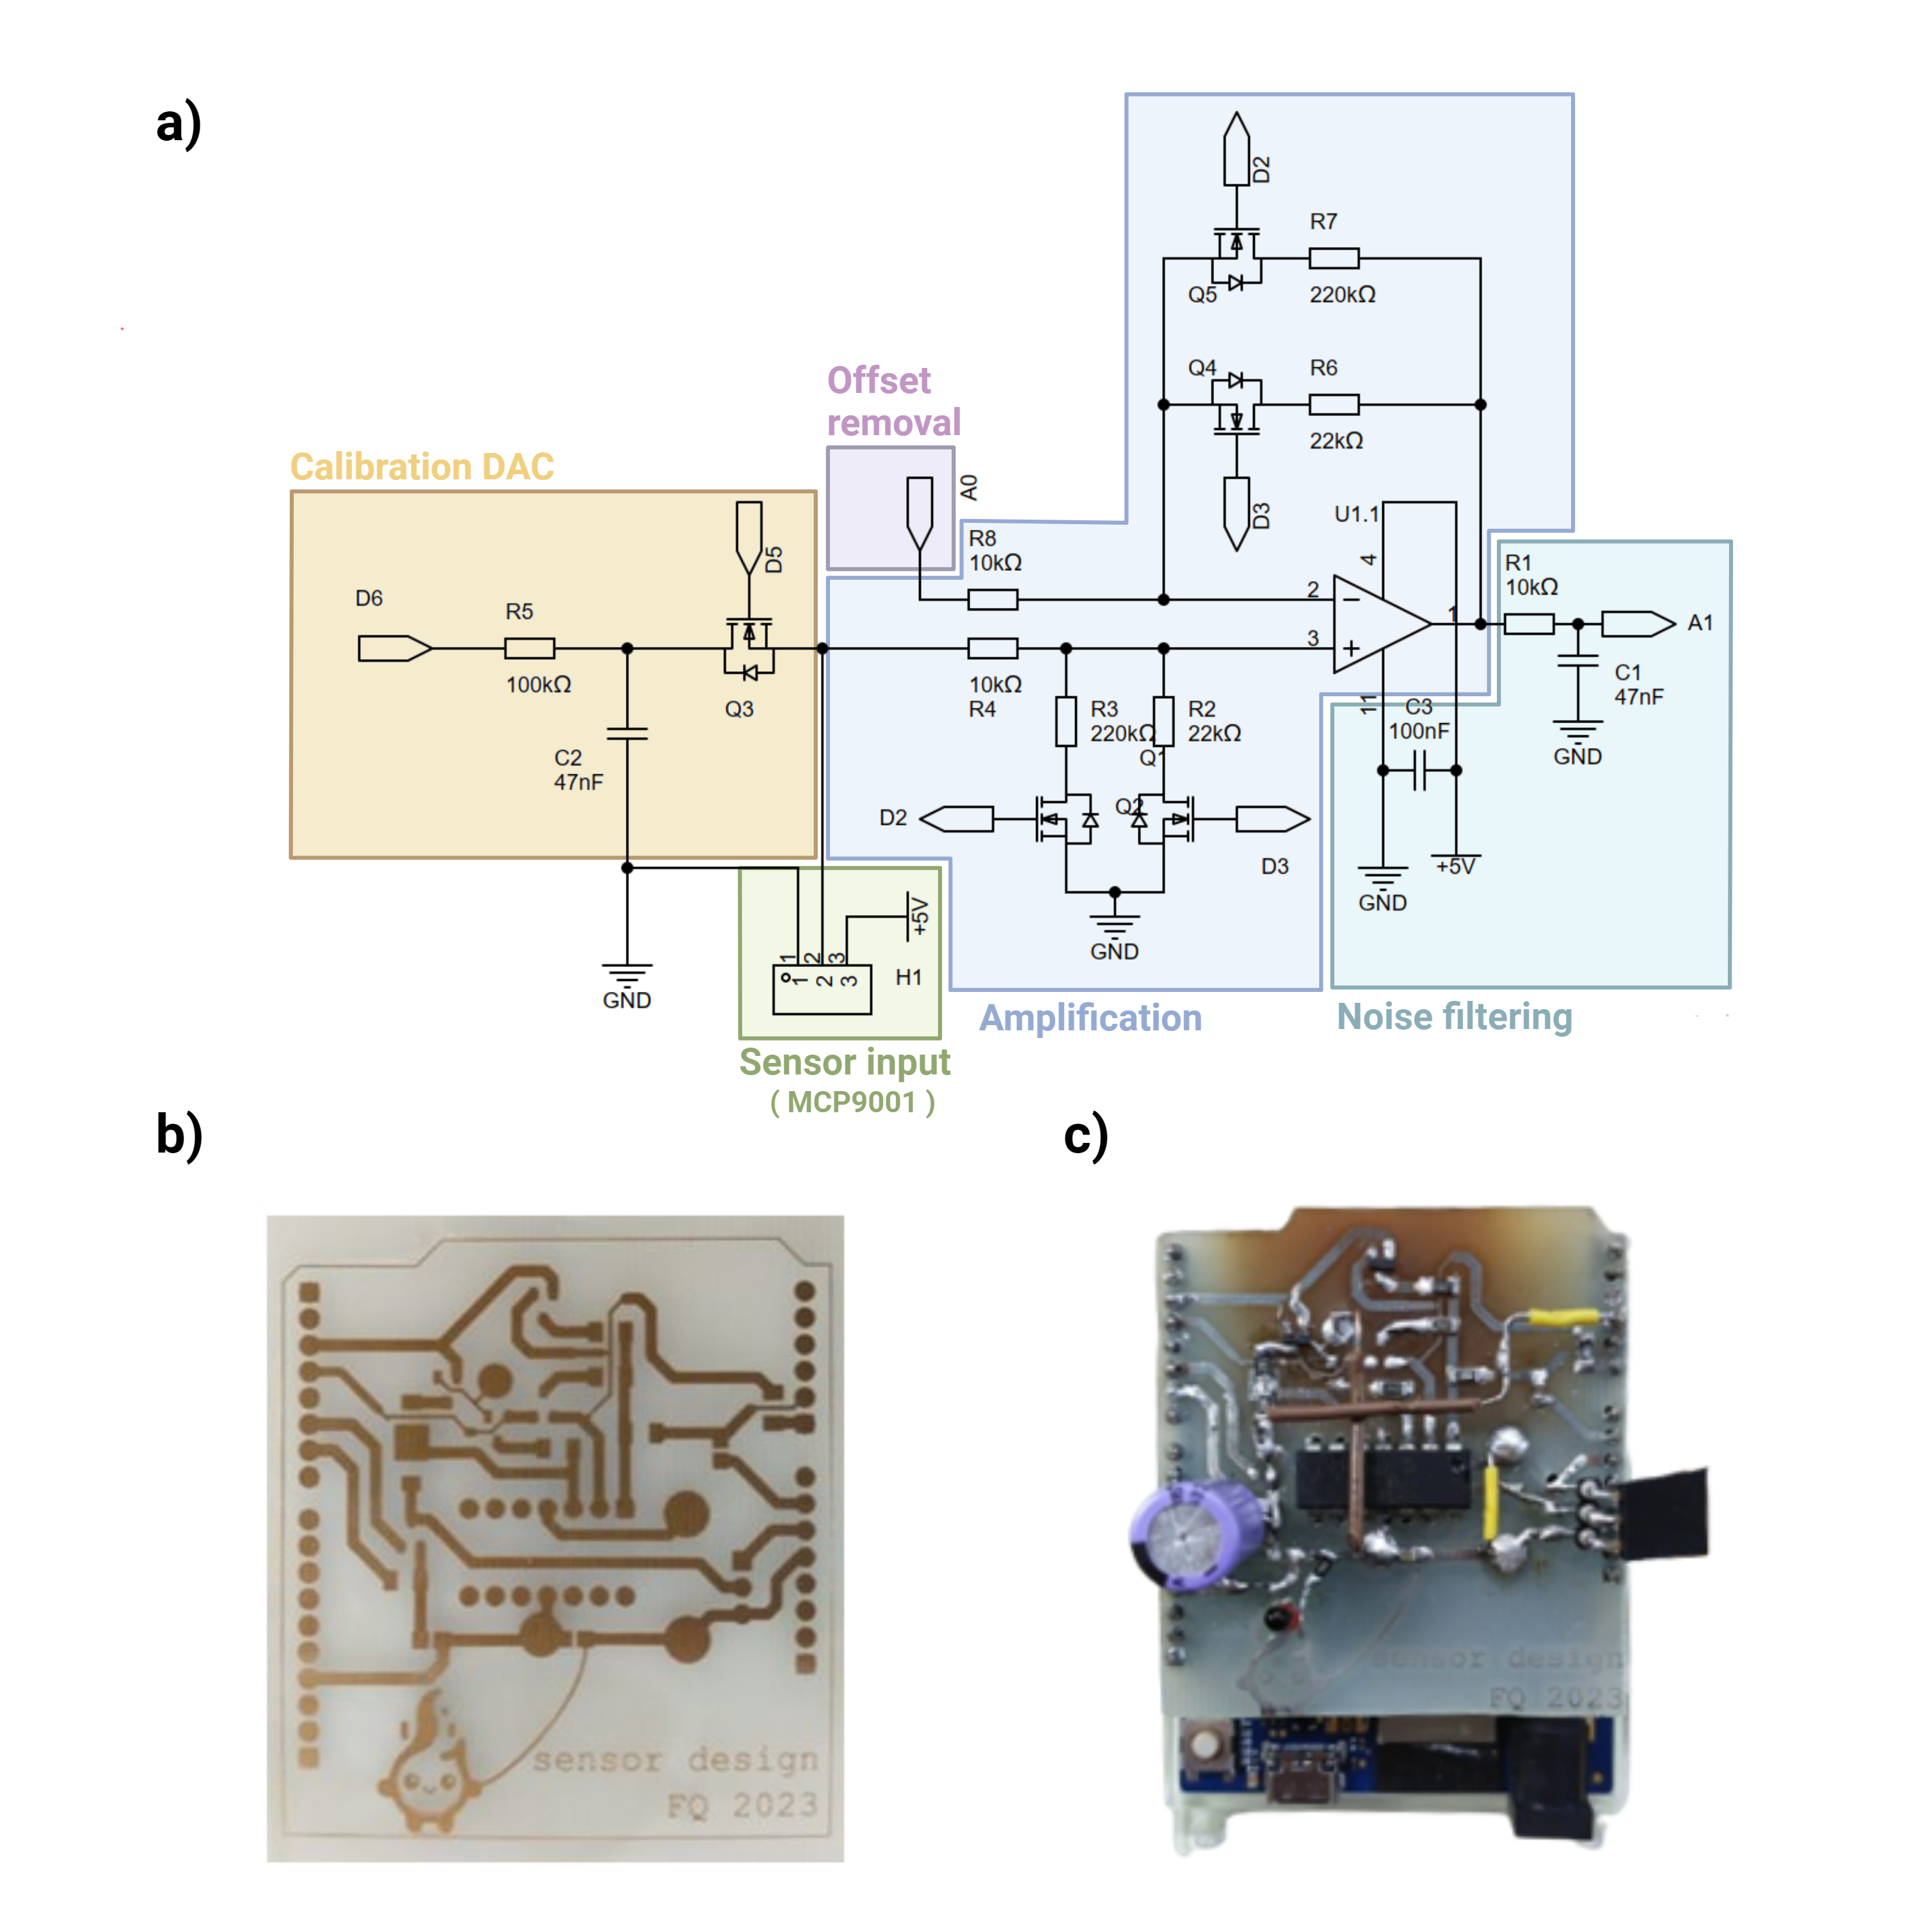
\includegraphics[width=\textwidth]{images/electronic_diagram.png}
   \caption{Annotated electronic diagram (a), etched PCB (b) and PCB after soldering and rework (c).}
   \label{fig:circuit}
\end{figure*}

   \subsection{Sensor design}
      \subsubsection{Electronic diagram}
         The complete circuit diagram is shown in Figure \ref{fig:circuit}. Overall, the designed circuit was divided into 4 parts:

         \begin{enumerate}
            \item A DAC module that converts the PWM current from the Arduino into a continuous voltage, which is fed into the positive 
               pin of the Operational Amplifier, simulating the voltages that the sensor will generate later. After experimental testing of
               the circuit and measuring it with an oscilloscope (results not shown), it was established that the resistance of the low-pass
               filter of the DAC should be as low as possible (100 Ohms finally) so that the relationship between its resistance and the
               rest of the rail (especially resistors $R_4 + {R_3} / {R_2}$) is low enough to obtain most of Vin at the output of the
               DAC (otherwise, a significant potential would drop across the DAC resistor). This circuit is connected or disconnected
               through the mosfet D5 (AO3400, Omega Semiconductor).

            \item The amplification circuit is composed of an operational amplifier (MCP9700, Microchip Technologies), working as a voltage amplifier in a range from 0 to 4.7V, and two MOSFET-based
               gain selection circuits, selecting gains of 2.2X or 22X. These circuits are activated with digital pins D2 and D3, and they change the close loop resistances
               and and another two mirroring ones on the non-inverting input that allows a 1:1 ratio in the offset removal.

            \item The offset removal, controlled through the Arduino's internal DAC on pin A0 with a precision of 12 bits and a range of 0-4.7V
               (when the Arduino is connected via USB), providing a theoretical step of 1mV. The offset is applied to the inverting input and undergoes
               the same type of resistance as the sensor voltage to apply a 1:1 subtraction.

            \item The noise filtering circuits, consisting of a 100nF decoupling capacitor and a low-pass filter at the output of the Operational
               Amplifier, which are responsible for filtering high frequencies from the microcontroller crystals, both in the voltage rail and at
               the output of the operational amplifier.

            \item The sensor connector, where the sensor is plugged into the system.
         \end{enumerate}

         % \clearpage

      \subsubsection{Electronics production}
      The circuit schematics were created in EasyEDA\cite{EasyEDAOnlinePCB}. The Arduino UNO Shield templates were imported from OpenSourceHardware Lab \cite{ArduinoShieldEasyEDA}.
      Printed circuit boards (PCBs) with pre-routed traces were printed on transparent projection films and aligned on a single-side copper board covered by a positive photomask.
      The PCBs were exposed to UV light for 5 minutes, followed by a sodium hydroxide bath to remove excess mask. Subsequently, the copper plates were immersed in a copper etchant solution (Ferric Chloride)
      to remove the copper from the exposed regions. Finally, the mask was removed with acetone, and the plates were immersed in thiourea to coat the copper with a layer of tin.
      \subsubsection{Sensor probe}
      The sensor was soldered to solid core wires and made waterproof using a combination of heat-shrink plastic and heat-shrink tubing. Two layers were added
      to ensure insulation, guaranteeing that the ceramic surface remained exposed to facilitate thermal exchange.
      \subsection{Sensor Calibration}
      To attempt to isolate the origin of any potential error, the operational amplifier was first calibrated (and its error studied), and then the output of the 
      operational amplifier was mapped against a digital reference temperature sensor (HH802WE, Omega).

      \subsubsection{Operational Amplifier Calibration}
      Initially, a voltage sweep was performed using the calibration DAC, from 0 to a saturation voltage (4.7V), first activating the gain 2 loop circuit and then the gain 22 circuit.
       After confirming that both circuits worked by comparing the obtained gains (and the amplification range) with the expected values, a "sequential offset subtraction" code 
       (using the Arduino's internal DAC) was implemented to subtract a discrete offset each time the operational amplifier was saturated (Appendix A; Figure \ref{fig:opamp}a). The results gradually show that as the 
       removed offset increases, a minimum in the output voltage is reached, beyond which the signal cannot decrease (Appendix A; Figure \ref{fig:opamp}b). The potential explanation for this voltage lies in the internal
        diode of the operational amplifier closed-loop MOSFETs. Even when the MOSFET is open, not conducting voltage through the loop from the output of the operational amplifier 
        to the inverting input, the internal diode of the MOSFET allows circulation from the inverted input of the op-amp to the op-amp's output, contaminating this output with the DAC voltage. 
        When the offset voltage is small, most of it falls on the diode, but as the output grows, it becomes more and more contaminated. Some specialized forums suggest using "back-to-back" MOSFETs\cite{BackBackMOSFET} 
        as a potential solution, but after a quick attempt, the result remained the same. Therefore, due to time constraints, it was decided to desolder the 2X loop and continue the experiment only with a 
        gain of 22, whose results, along with the offset subtraction script, showed an effective input range from 0 to 4.7 volts with an output (including the subtracted offset from the sensor voltage) 
        of approximately 0-104V (Figure \ref{fig:finalop}).

        \begin{figure}[!th]
         \centering
         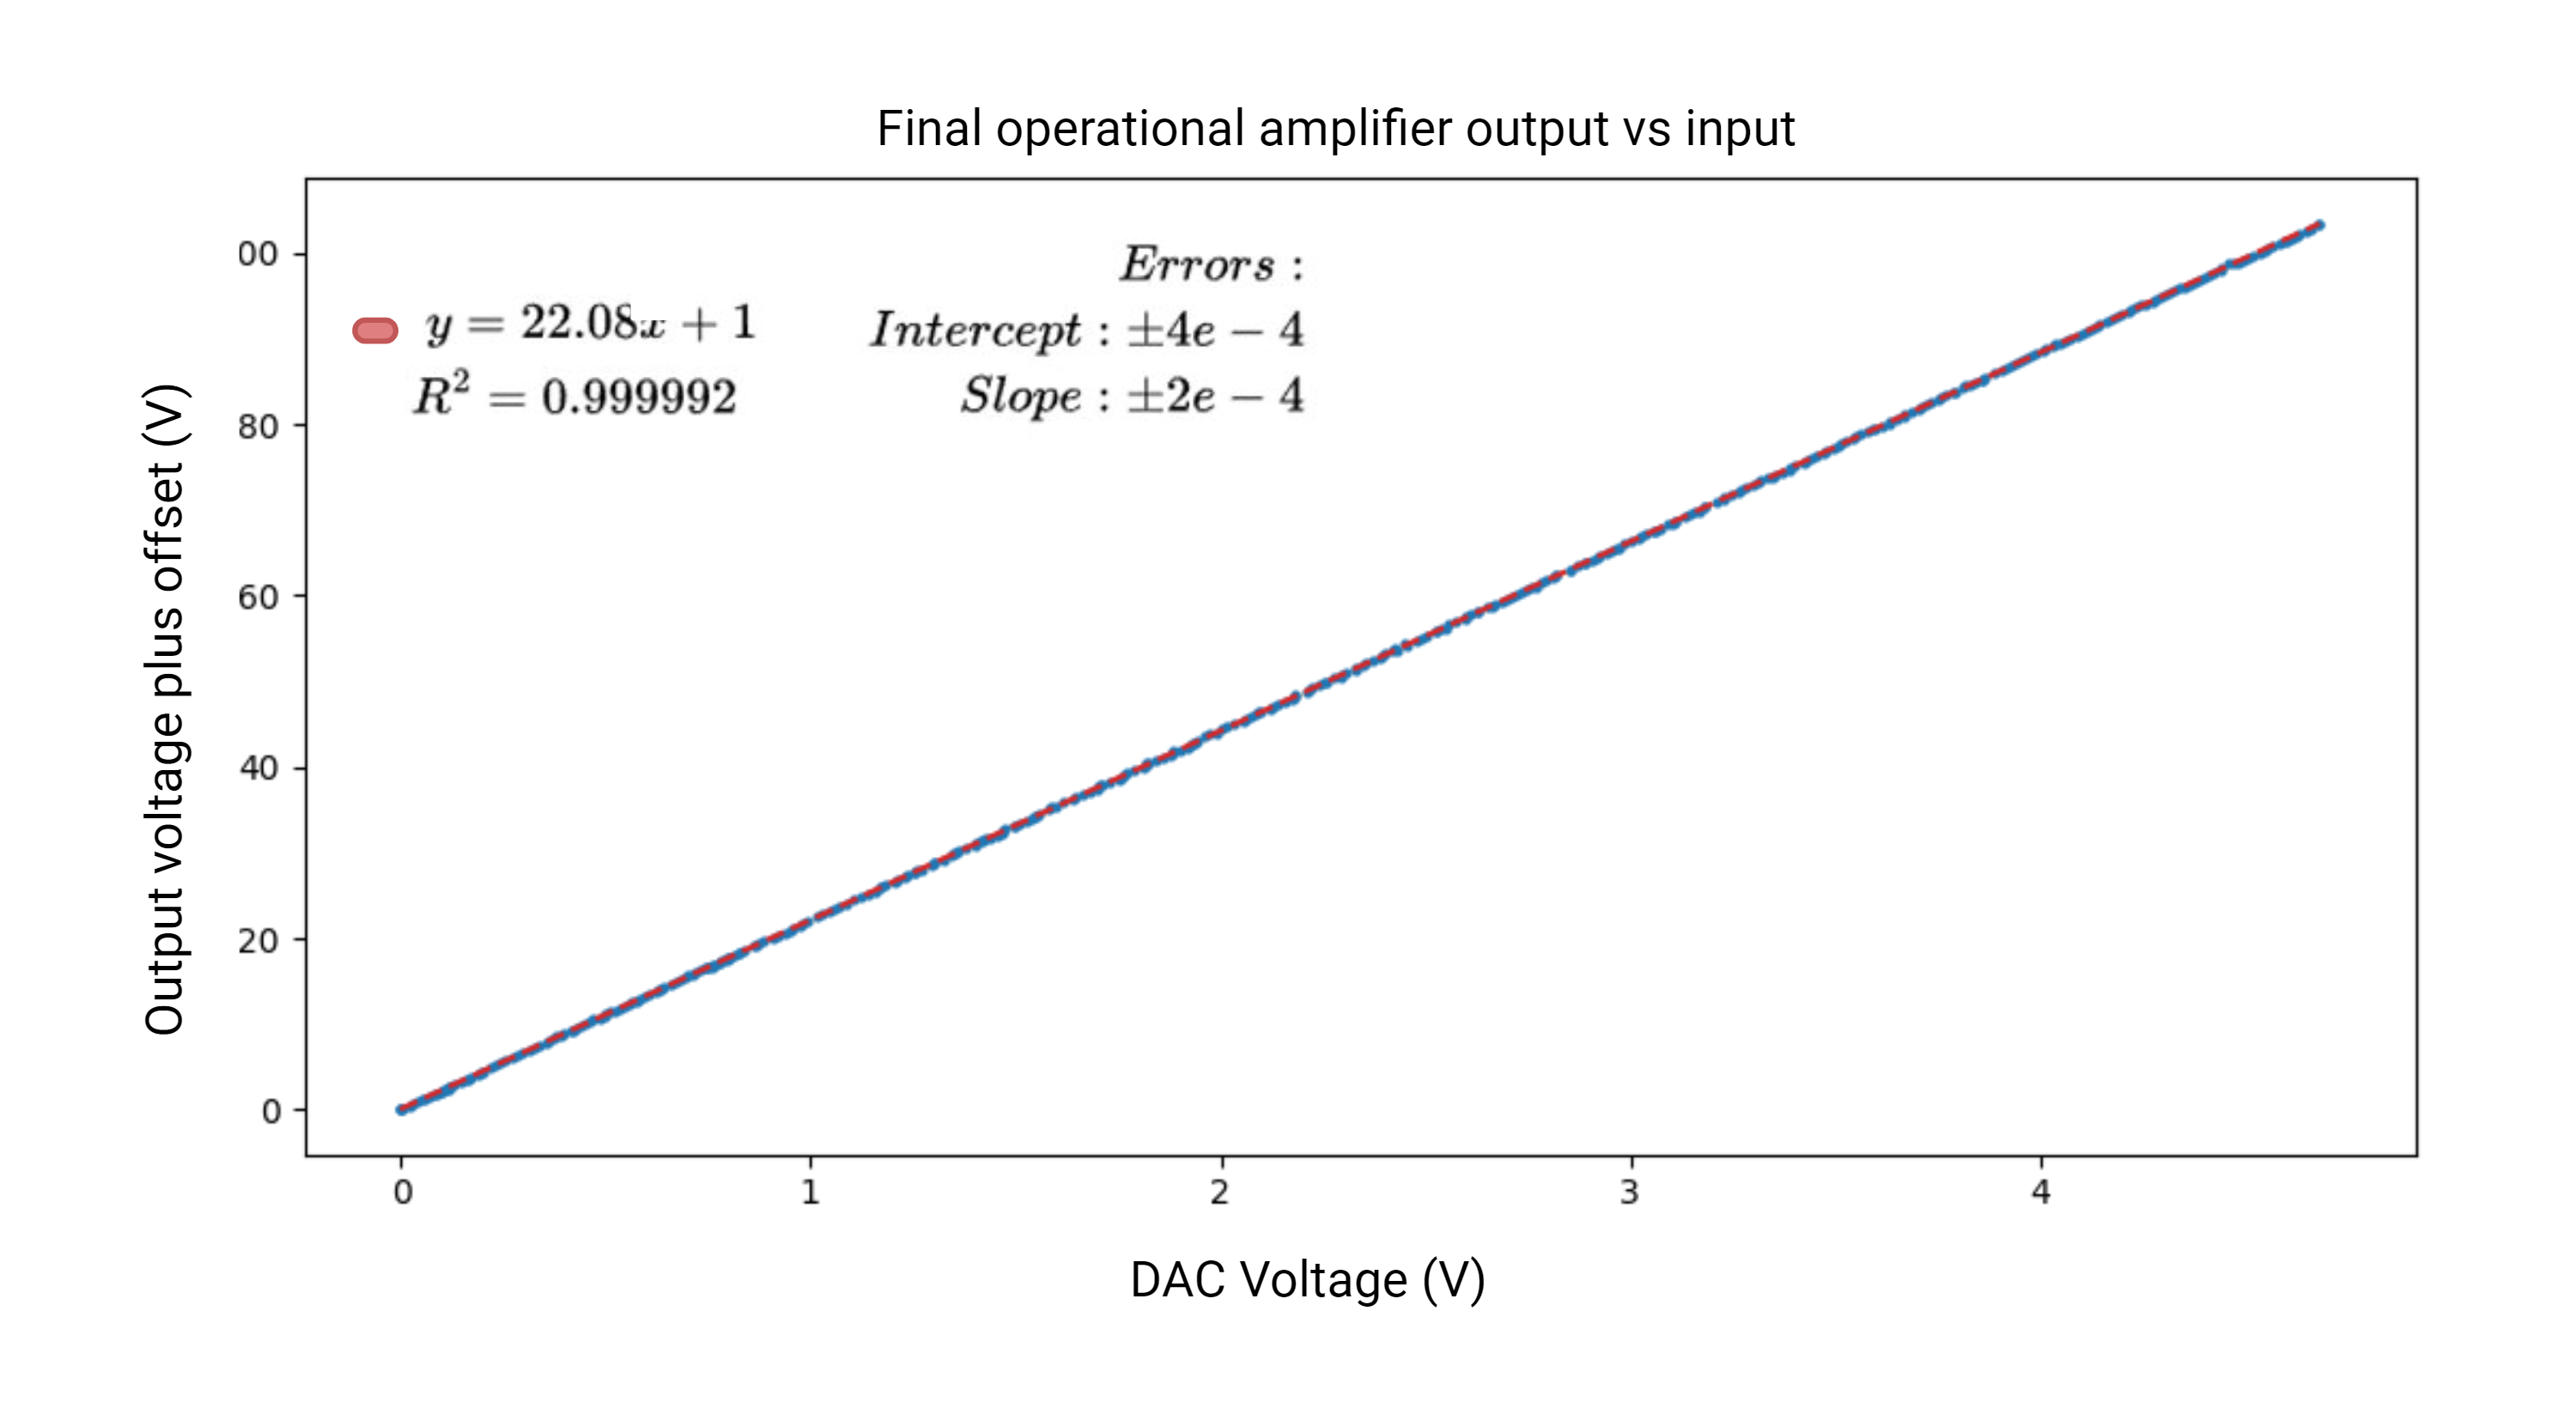
\includegraphics[width=1\linewidth]{images/finalop.png}
         \caption{Output response operational amplifier voltage after adding the offset.}
         \label{fig:finalop}
      \end{figure}

      \subsubsection{Temperature calibration}

      For temperature calibration, a previously published open-source isothermal fluorimeter was modified \cite{Open_qLAMPMasterOpen2023}.
      The heated lid was separated from the housing and folded around the two sensors, creating the equivalent of a 'spring roll' with the two sensors 
      in the center and the lid spiraling around them (Figure \ref{fig:temp}a). The lid was then heated at different temperatures, after which it was allowed to reach thermal 
      equilibrium for 3-4 minutes, and the voltage value at the output of the operational amplifier and the temperature of the reference sensor were recorded. 
      A linear regression was then established, and confidence intervals were calculated, resulting in a maximun error ~±1°C (Figure \ref{fig:temp}b).
      
      \begin{figure}[h]
         \centering
         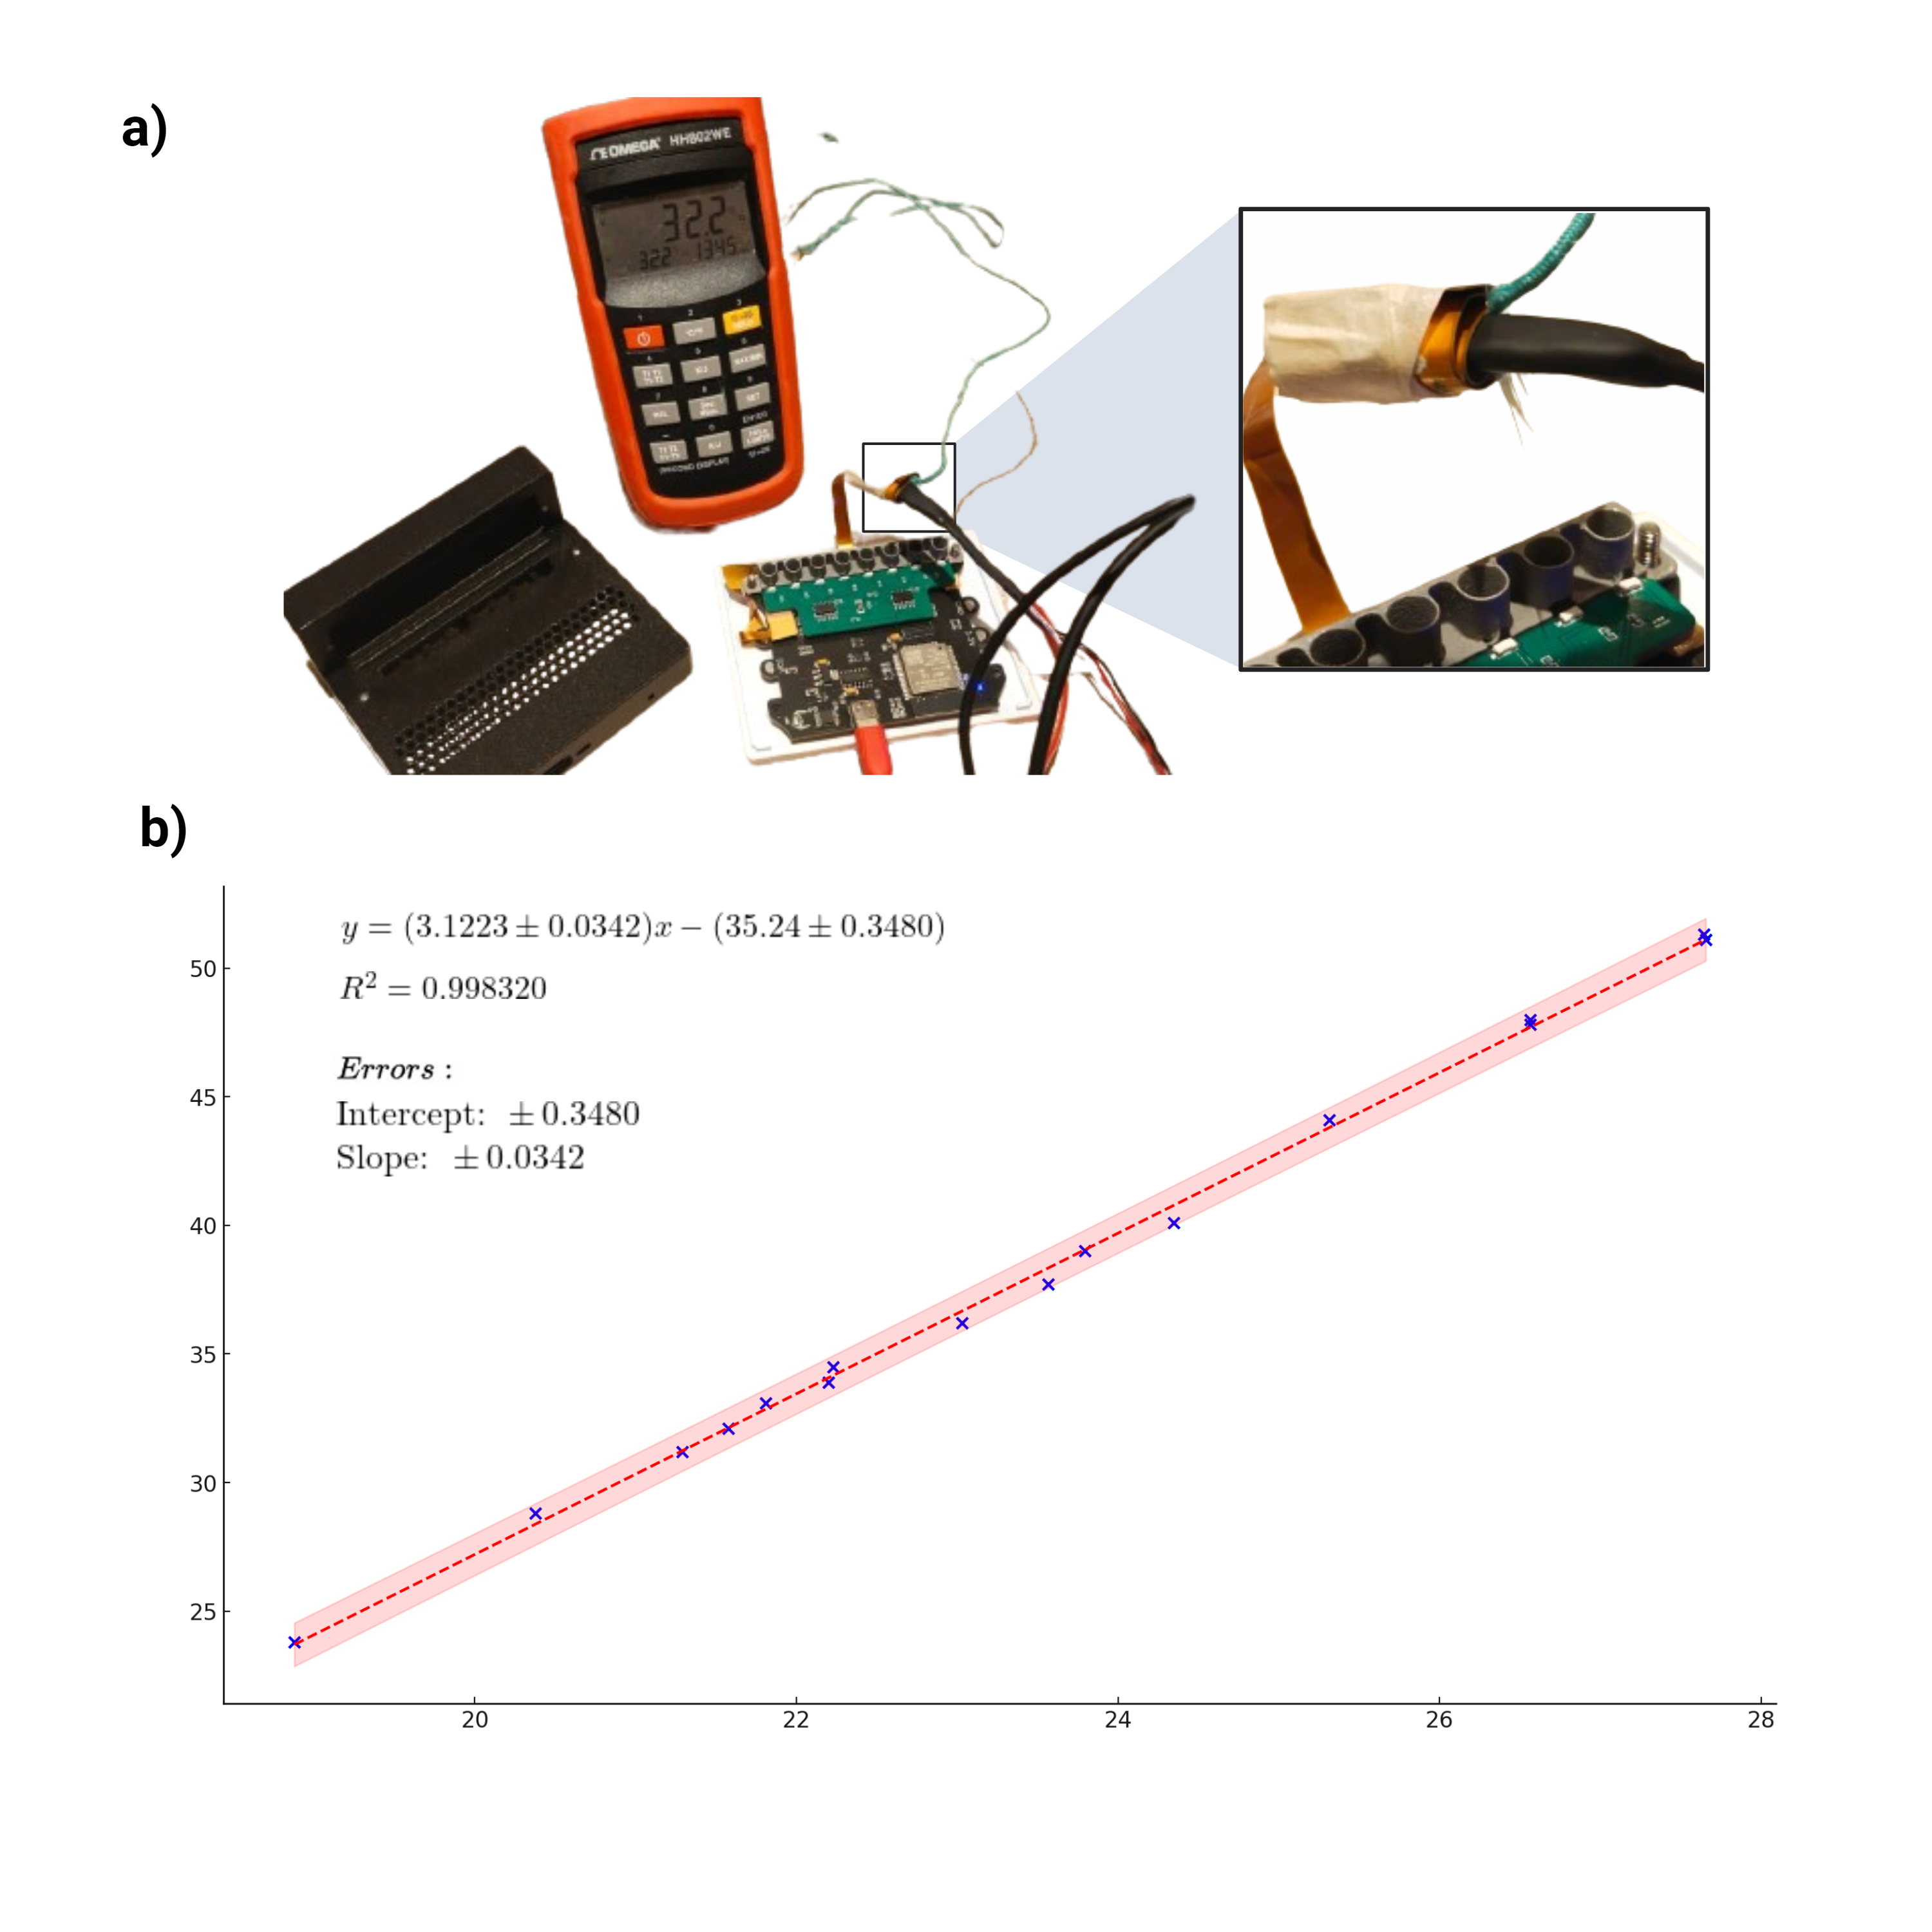
\includegraphics[width=1\linewidth]{images/temp calibration.png}
         \caption{Temperature calibration setup (a) and results (b)}
         \label{fig:temp}
      \end{figure}


      \subsection{Results and discussion}

   Finally, the sensor was tested against the reference method to measure a dynamic system, the cooling of freshly boiled water from 95°C to 25°C. Both sensors were coiled together and secured with thermally conductive tape. 
   They were submerged in the water, and the temperature was continuously recorded and plotted with a linear correlation analysis (Figure \ref{fig:final}).

   \begin{figure}[h]
      \centering
      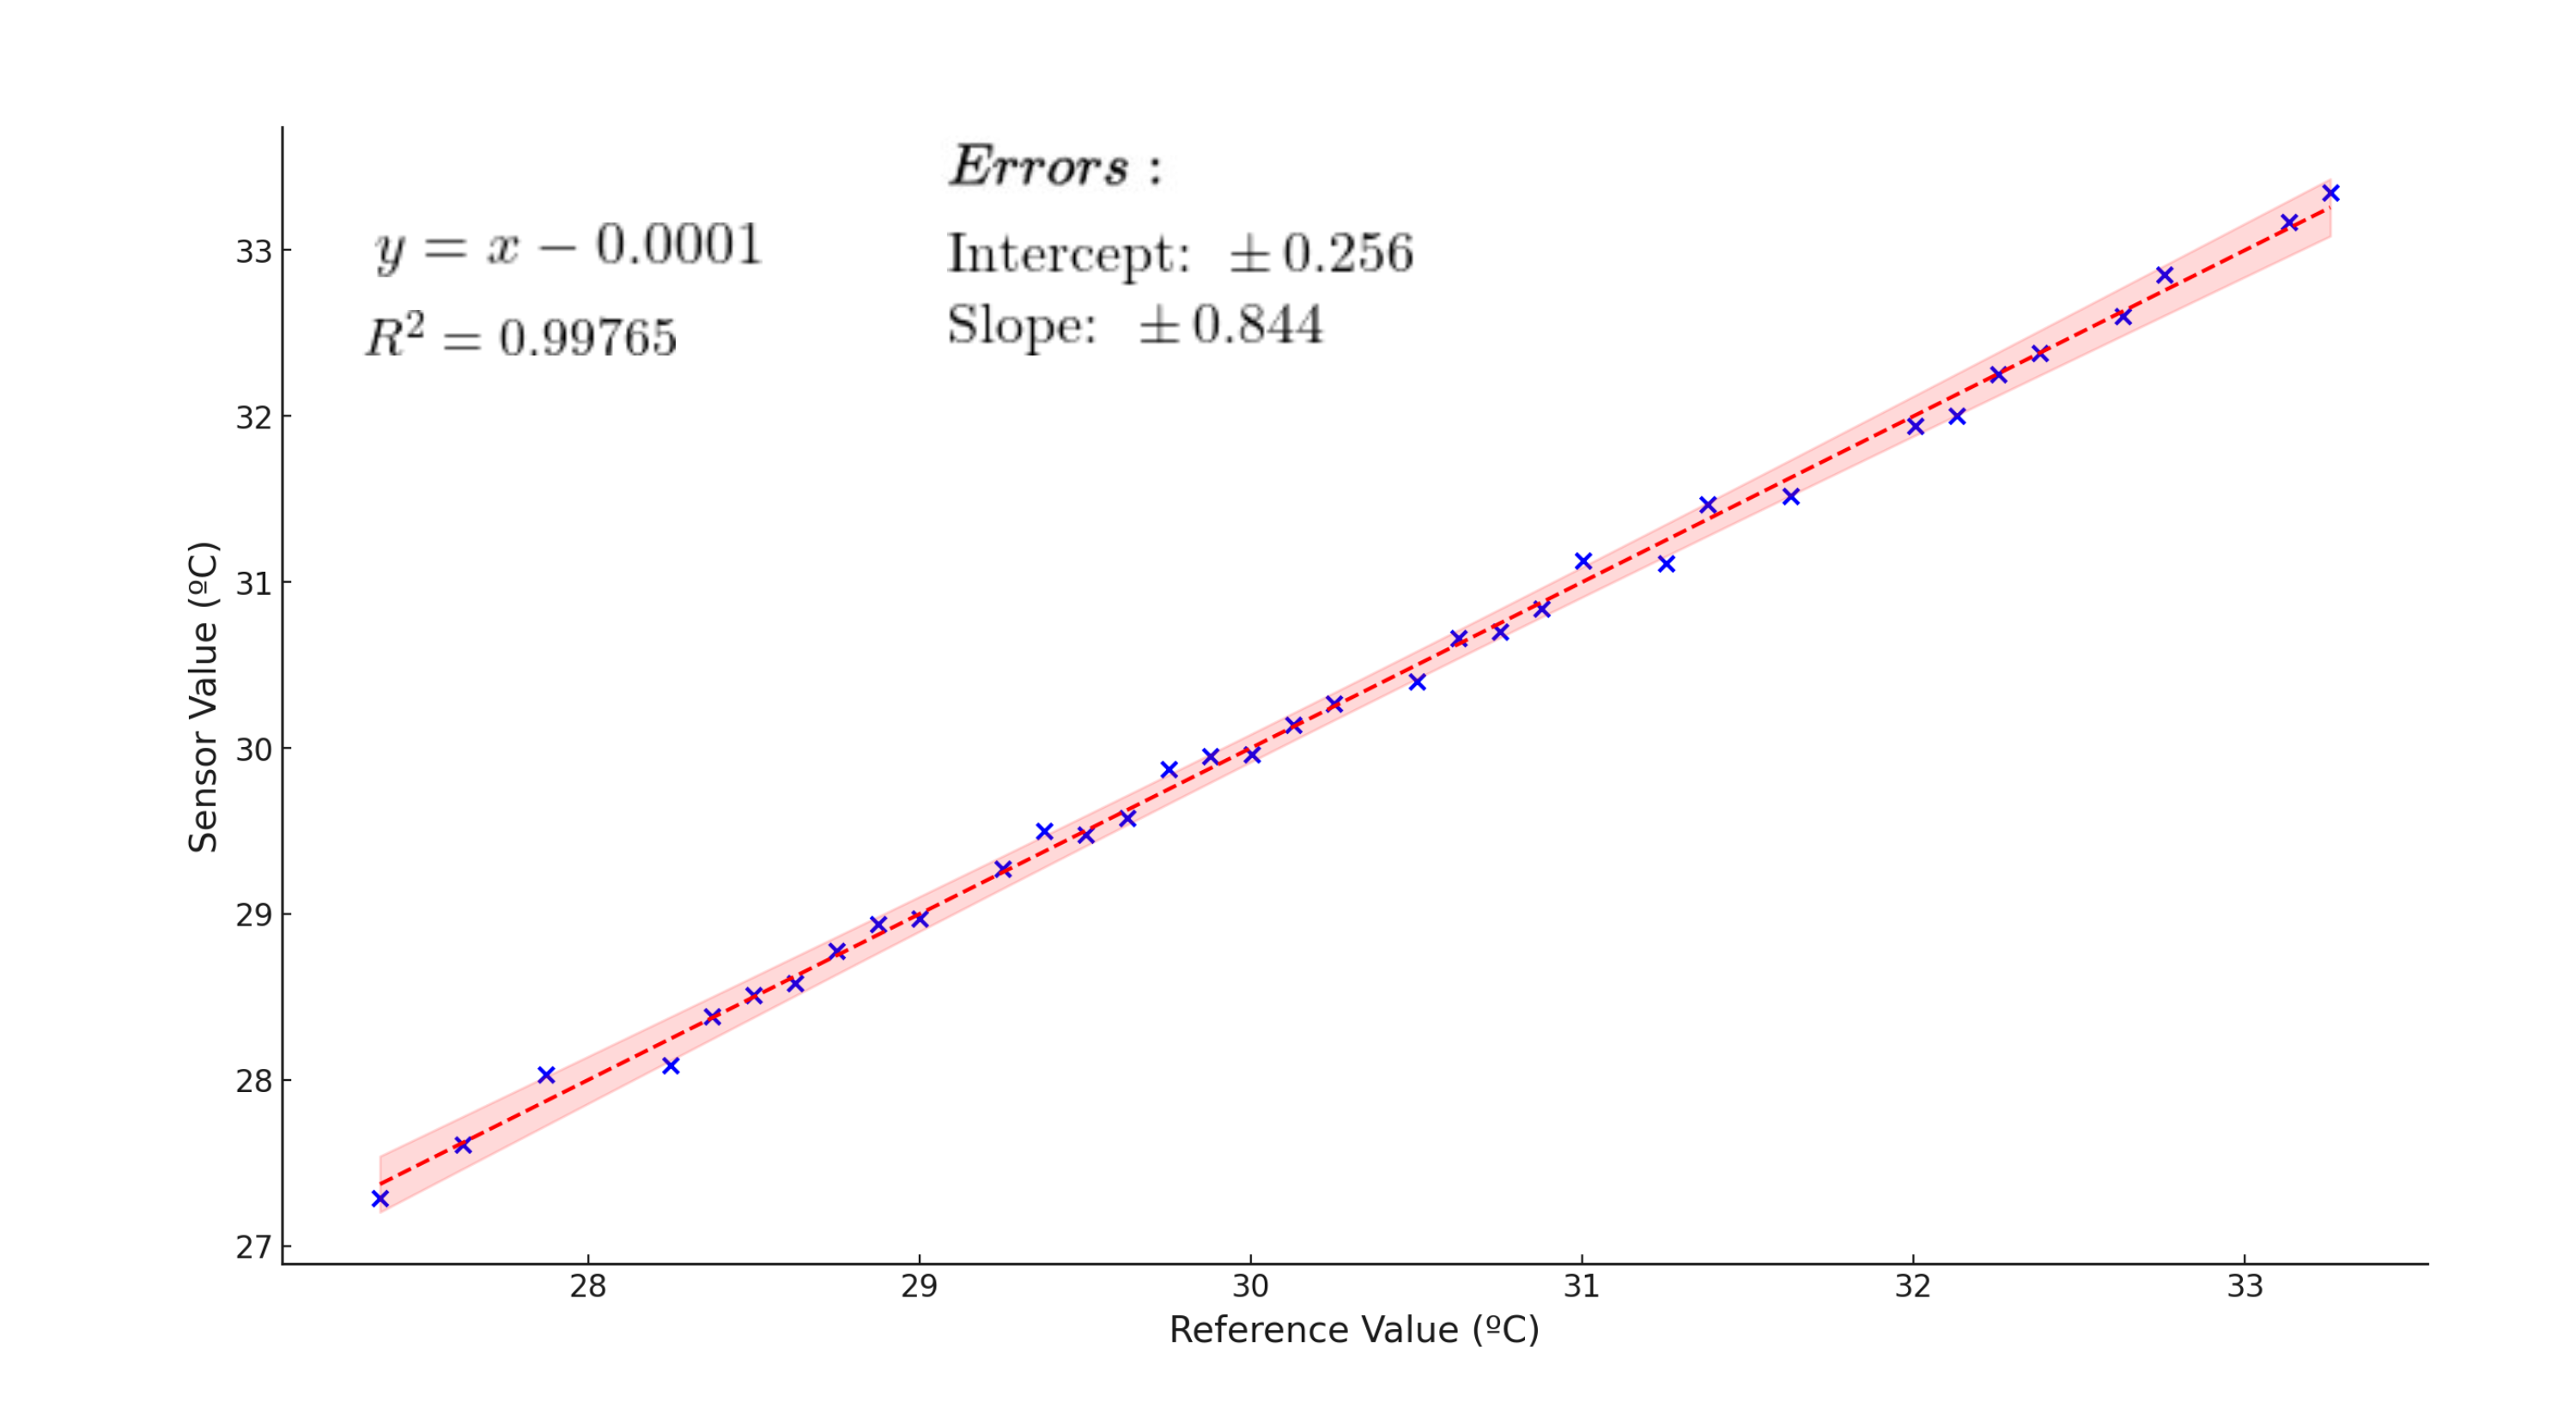
\includegraphics[width=\linewidth]{images/final results.png}
      \caption{Calibration results and linear regression (a), and Bland-Altman plot of residual distribution (b).}
      \label{fig:final}
      \end{figure}
      
      From these results, several observations can be made:
      
      \begin{enumerate}
      \item Both methods demonstrated an strong 1:1 correlation with an R-squared value close to 1, a slope of 1, and an intercept almost equal to 0.
      \item The residual distribution, as shown in the Bland-Altman plot, reveals a maximum difference between values of approximately ±1°C (accuracy of ~±1°C). Additionally, within the physiological range (32ºC-40ºC), the maximum error is about ±0.4ºC. This error seems to negatively correlate (decreasing with temperature) up to 40ºC, suggesting the potential for applying an additional linear correction within this range to further enhance accuracy.
      \item Considering the negligible error from the operational amplifier during calibration and the fact that the final error closely matches the sensor calibration against the reference method, it is evident that the replicability of the MCP9700 readings is the primary factor limiting accuracy improvement. 
      Interestingly, the error in the final dynamic system is less than that in the calibration experiment. This may be due to less thermal uniformity in the calibration experiment, 
      where the reference sensor was coiled around the sensor being calibrated, touching the metallic walls of the heater (and thus subject to direct temperature changes) while the 
      sensor being calibrated, surrounded by a much thicker ceramic layer, took longer to absorb and release immediate changes from the heater.
      \item The results from the adaptive offset circuit are satisfactory, allowing for potentially higher amplification gains than 22 without limiting the range. However, given the accuracy results of the sensor and the source of variability, increased amplification does not appear to be the limiting factor.
      \item Finally, these results indicate an improvement from the ±2ºC accuracy specified in the component's datasheet to ±0.4ºC in the physiological range, representing a fivefold improvement. 
      
      \end{enumerate}

\section{Pulse meter} % 1000 words
   \subsection{Introduction and goals}
   The aim of the pulse meter section was to understand the principles and mechanisms of sensor designs with a `hands-on’ approach. In particular, here we built a DIY pulse meter. 

   There are two possible main mechanisms behind pulse meter design, both relying on the use of a warm light (red). In the `transmission’ design, the LED is placed on the top of the finger, and the light transmitted is detected at the bottom; the ‘reflection’ design instead places the LED and the sensor close to each other, with the sensor detecting the amount of light reflected. Here, we chose to implement a reflection pulse meter for simplicity, as it allows for placing the LD and the sensor on the same PCB. 
   
   Three main steps were taken in the design and testing of our prototype: (1) sensor and (2) mechanical designs, followed by (3) the software part development.
   
   \subsection{Sensor design}
      \subsubsection{Hardware subsystems}
      The electronic design was constructed following the provided design of a circuit with a transimpedance amplifier followed by a voltage amplifier.
      Only the following modifications were included (Figure \ref{ed2}):
         - The MOSFET U2 (AO3400, Omega Semiconductor), to bypass resistor R3 and facilitate the rapid charging of capacitor C2. The goal is to temporarily activate this fast charging to allow the circuit to adapt
         more quickly to changes in DC offset.
         - The LEDs and photodiodes were externalized on a separate PCB to allow for better positioning. Through-hole components were replaced with SMD components (as they provide better skin contact),
         and two photodiodes were placed in series to improve the signal.

      Unfortunately, the photolithography system was not available during the week when the PCBs needed to be produced, so all PCBs were hand-drawn with a permanent marker on double-sided copper plates.
      Subsequently, the copper plates were immersed in a copper etchant solution (Ferric Chloride) to remove the copper from the exposed regions. Finally, the mask was removed with acetone, and the plates were immersed in thiourea to coat the copper with a layer of tin.

      \begin{figure}[t]
         % \afterpage{\clearpage}
         \centering
         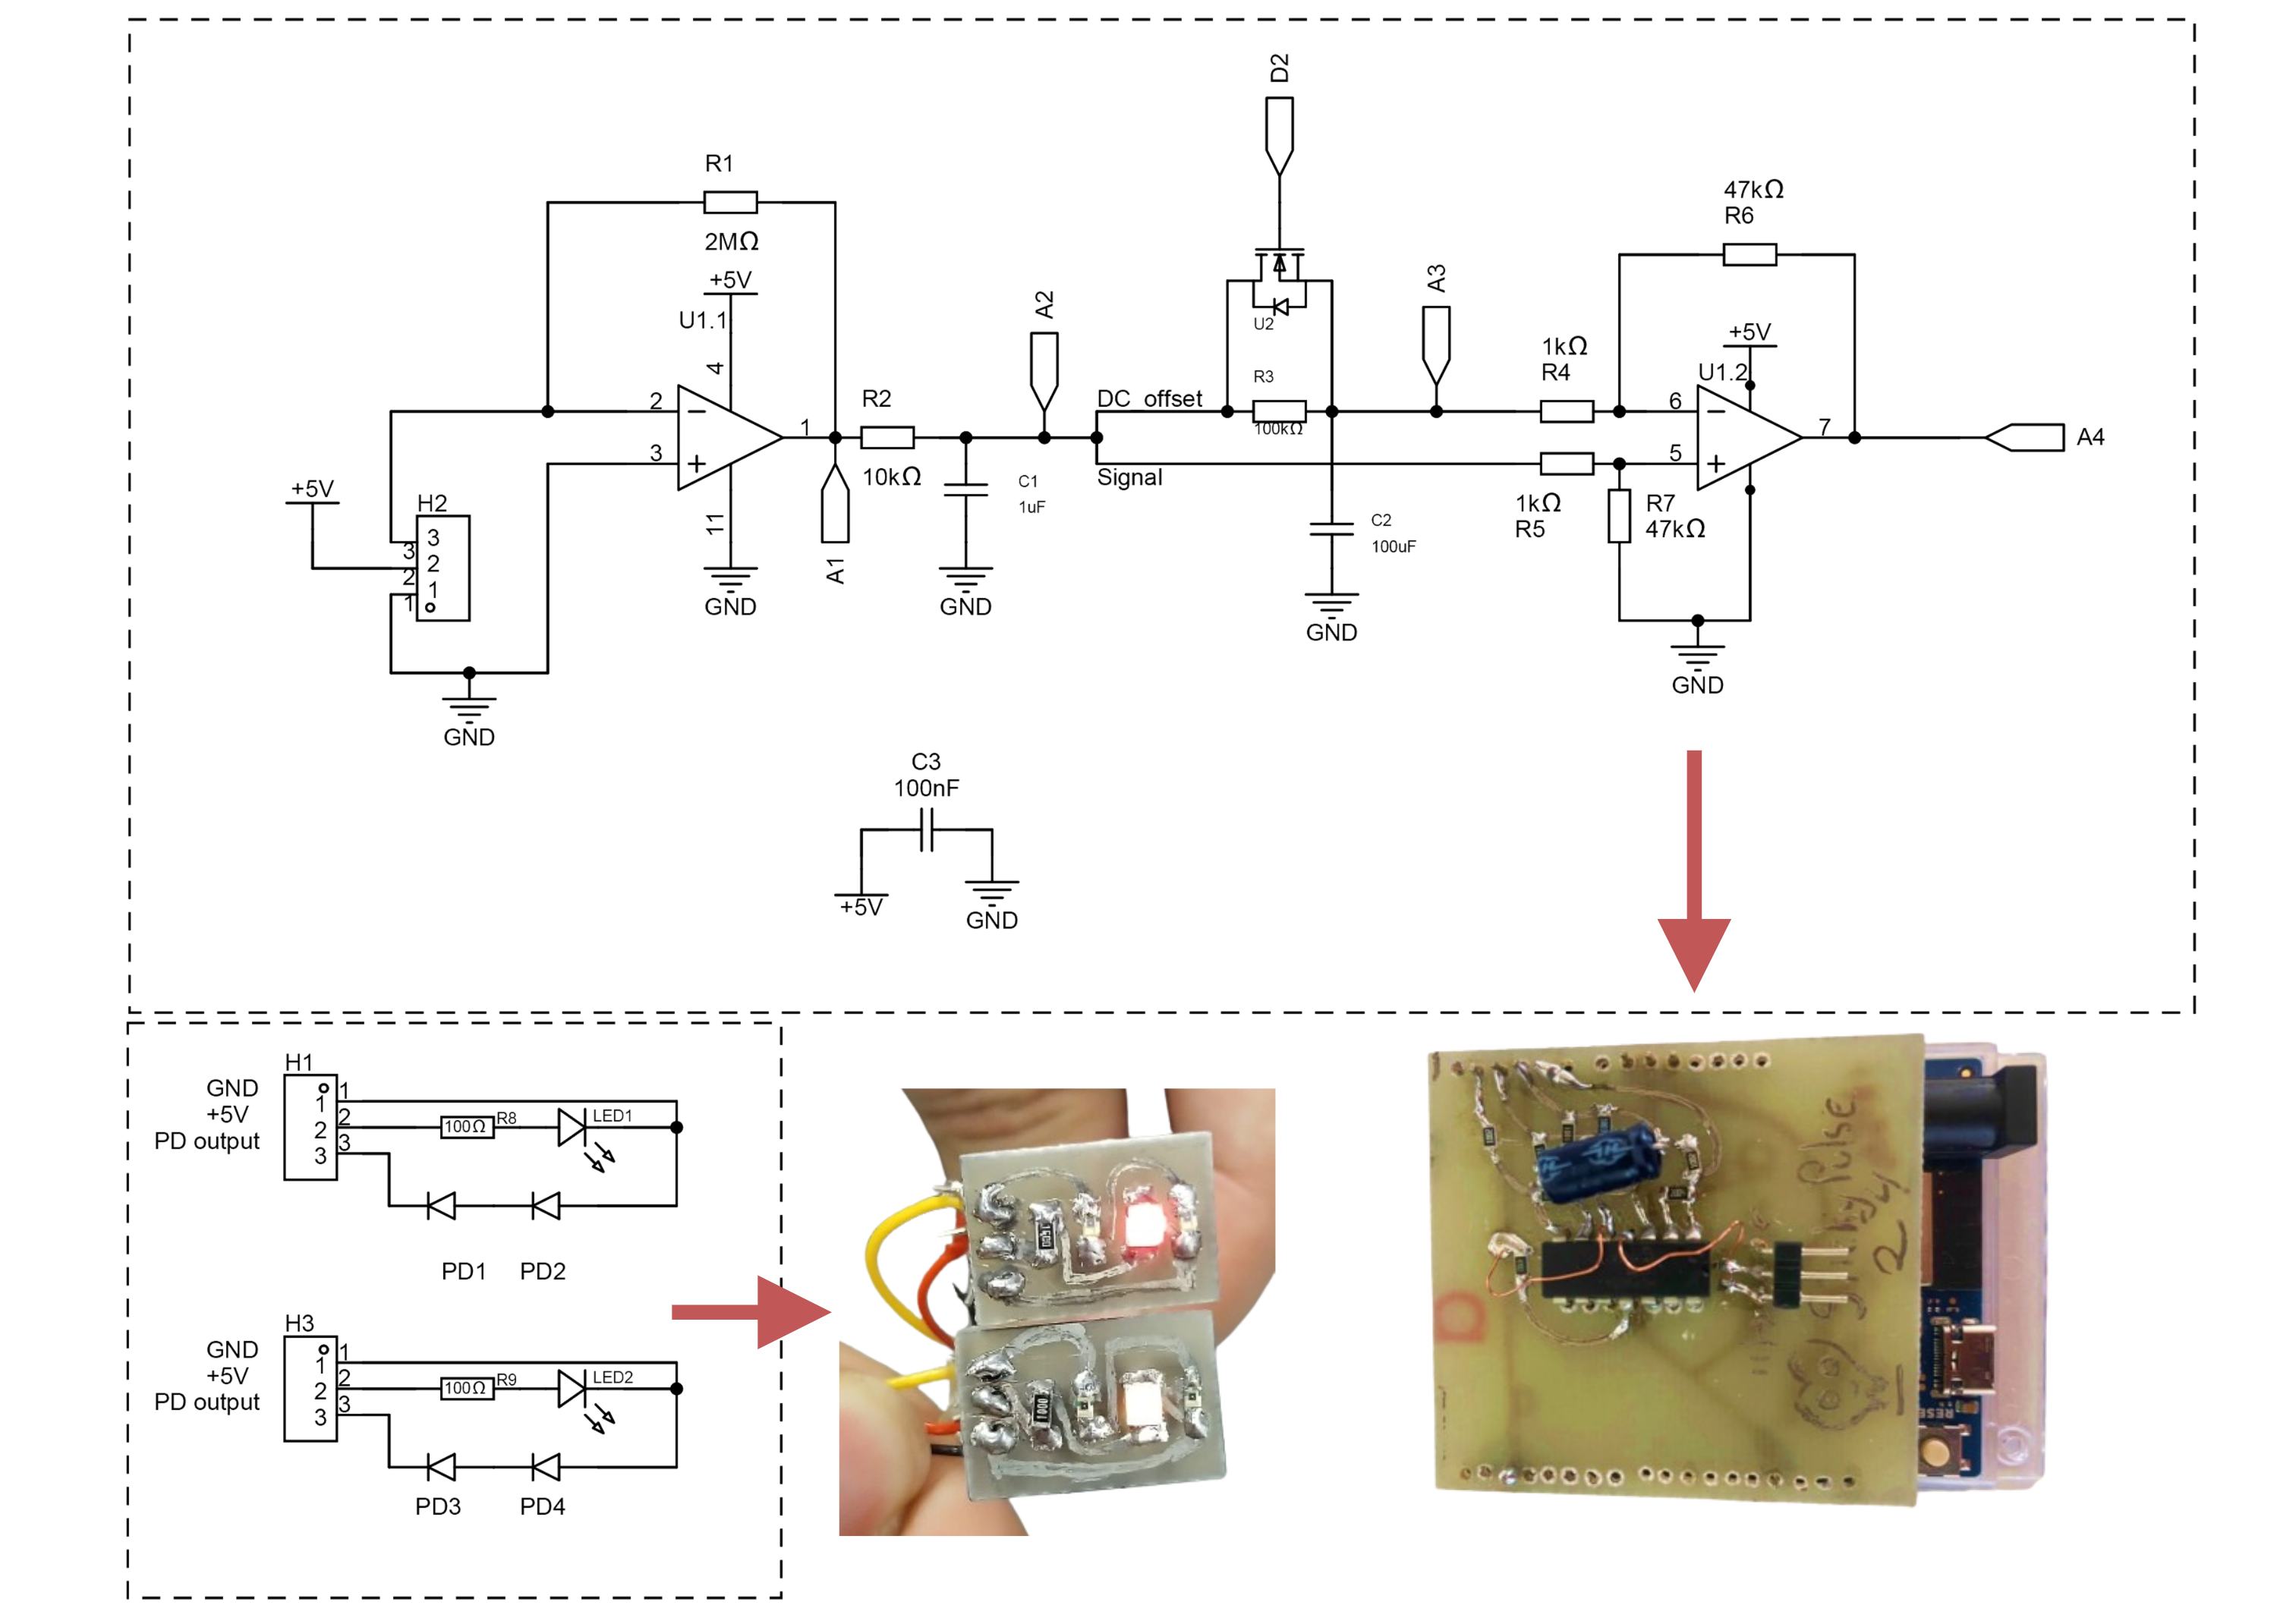
\includegraphics[width=\linewidth]{images/ed2.png}
         \caption{Annotated electronic diagram (a), etched PCB (b) and PCB after soldering and rework (c).}
         \label{fig:ed2}
      \end{figure}
      \subsubsection{Mechanical design}

      Two components were designed and produced by 3D printing. The first is the \textbf{sensor probe holder}, fixing the sensor in position while reducing  as much mechanical noise as possible; the second is the \textbf{case} that holds and protects the main electronics, and the battery to make the system portable (Figure \ref{fig:mec}). 

      We developed and tested \textbf{two different sensor probes} (Figure \ref{fig:mec}): we called them `sticky pulse’ and `touchy pulse’.  Touchy pulse is designed as an envelope surrounding the finger while holding the sensing PCB pressed against its bottom: such a  pressure is ensured by a thin spongy layer inside the envelope itself.
      Sticky pulse design consists instead of a plastic flexible piece holding the PCB, meant to be sticked at the location where pulse has to be recorded. 
      
      While touchy pulse allows for recording only on the finger, with sticky pulse we could experiment at different locations. The better signal (i.e more amplitude) was achieved near the jugular vein of the neck, potentially because of the higher blood flow at this point. Although sticky pulse allows for more flexibility and better signal when correctly placed, it also has the drawback of being more sensitive to mechanical noises (as speaking or deglutition). Finding the correct point at which to stick can also not be straightforward. Touchy pulse presents a less neat signal, but is less prone to be affected by mechanical noise and it’s more user-friendly. 
      
      \textbf{The case} is a rectangular piece embedding the Arduino. A spiral is attached to its lateral part, holding a 5V external battery.
      
      \begin{figure}[!b]
         % \afterpage{\clearpage}
         \centering
         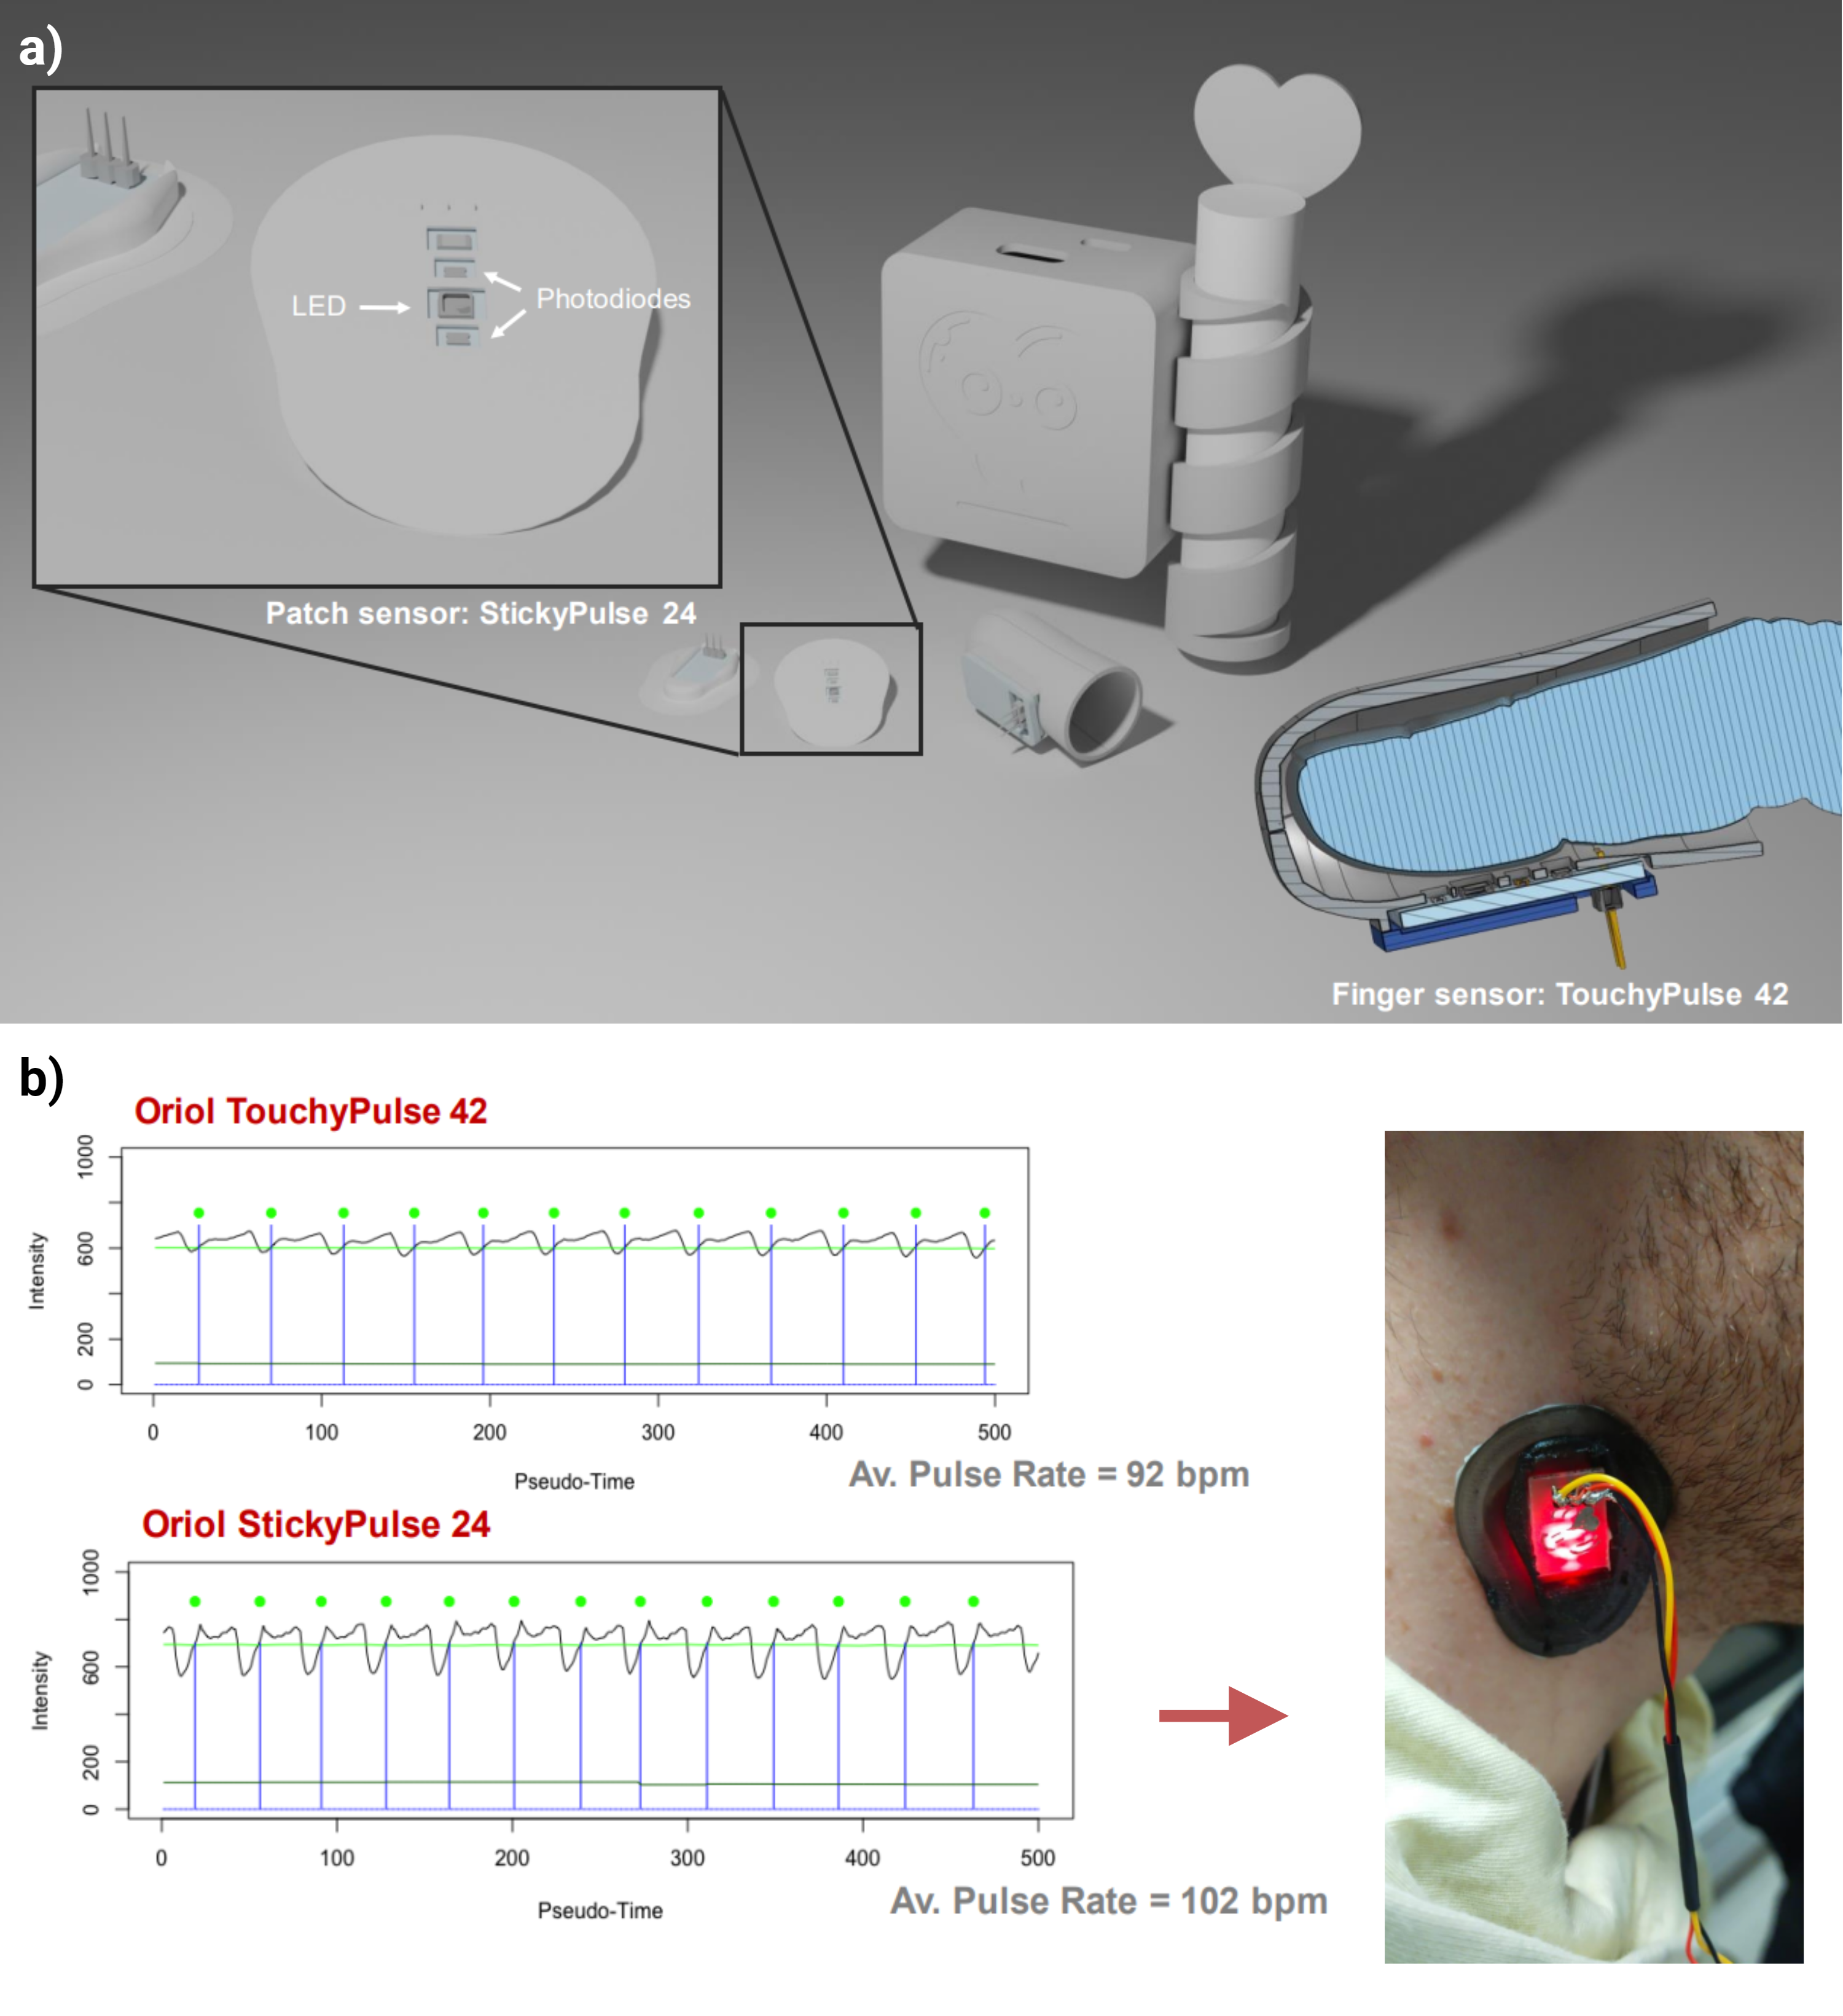
\includegraphics[width=\linewidth]{images/mechanical design.png}
         \caption{(a) Render of the mechanical components of the pulse meter (case, sticky and touchy pulse). (b) Comparision between touchy and sticky pulse.}
         \label{fig:mec}
      \end{figure}

      % \subsubsection{Case}
      \subsubsection{Software subsystems}
      The software is divided into three subcategories: 

      \begin{figure}[t]
         % \afterpage{\clearpage}
         \centering
         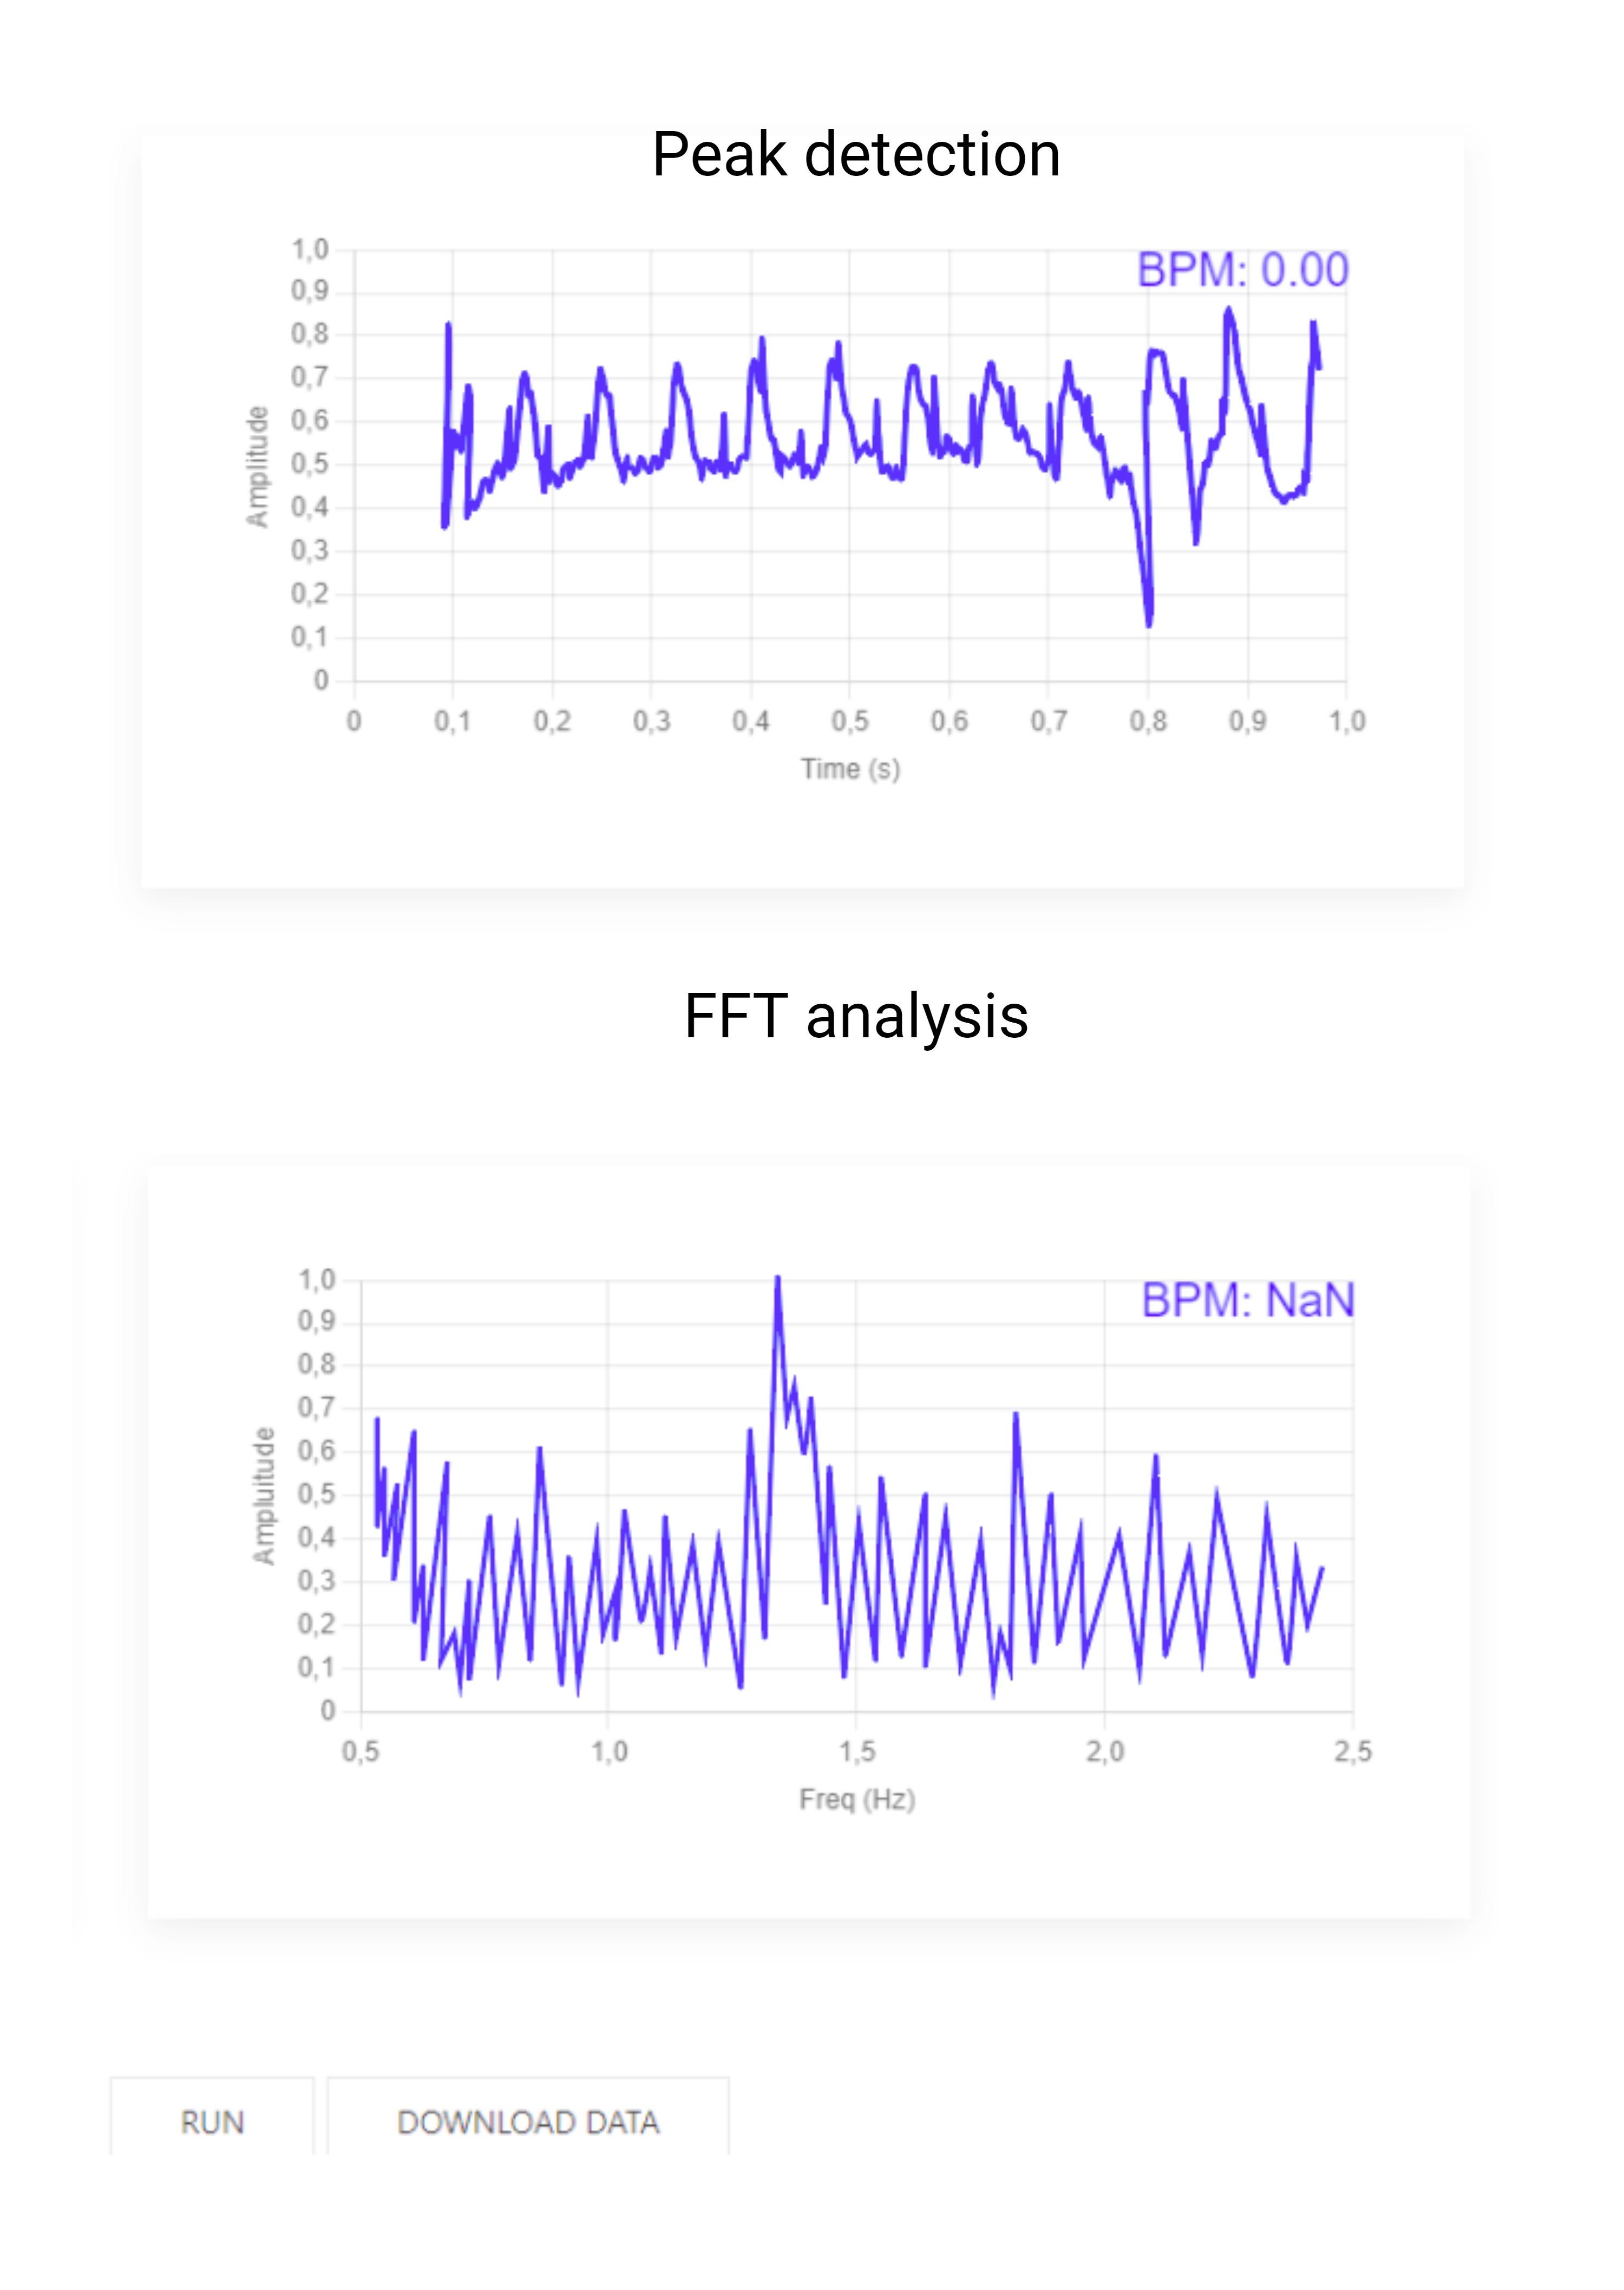
\includegraphics[width=\linewidth]{images/mockupweb.png}
         \caption{Screenshot of the JavaScript webpage results with peak analysis and FFT, locally computed by the device running the webpage. We addressed to display the results, but the BPM computation based on them is not yet implemented.}
         \label{fig:webpage}
      \end{figure}

      \textbf{Embedded system}: the Arduino code is divided in two main loops, each of them consisting in two different states of the Arduino protocol - signal measurement and data transmission. 
      
      In the signal measurement step, the Arduino reads 1000 values of the transimpedance circuit without any delay. In this phase, it rejects any request for data. After this, the transmission part is allowed and the Arduino waits for clients to request data. Once data are sent, it goes back to the first state.
      
      For \textbf{signal analysis}, we implemented two different protocols. The first is based on \textbf{peak detection} and the second on \textbf{Fast Fourier Transformation (FFT)}. In the peak detection protocol, the first step is the computation of the moving average of the signal: this value is then used as a threshold to define and detect the peak. Subsequently, the time between the peaks is computed to calculate the beats per minute (BPM). The last step is error filtering: here, aberrant peaks are removed by looking at the time between them - i.e peaks anomalously close are likely due to technical errors. 
      
      In the FFT protocol, we first remove the moving average from the signal to subtract any remaining DC offset; then, we compute the FFT signal between 0 and 2.5 Hz. The highest peak is then taken to compute the BPMs.
      
      
      Just the first peak detection method was validated in Python, but we ran out of time to validate the second one in Python due to time constraints. We then moved on to implement them on the JavaScript user interface: while the coding part was completed, and both methods were implemented, we unfortunately did not have the time to do the characterization of analysis on-the-go.  
      
      \textbf{User interface}. We coded the user interface with HTML and JavaScript, and embedded it inside the Arduino code. Once a device (as a smartphone) is connected to the same local network as the Arduino, it can perform a GET request to the Arduino, which will in turn send the webpage. Arduino then starts the two-state loop described above (measuring/transmitting data), while the computer runs the webpage locally, constantly requesting for data and performing the two analyses (peak detection and FFT) on its own (Figure \ref{fig:webpage}).
 


      \begin{figure}[!b]
         % \afterpage{\clearpage}
         \centering
         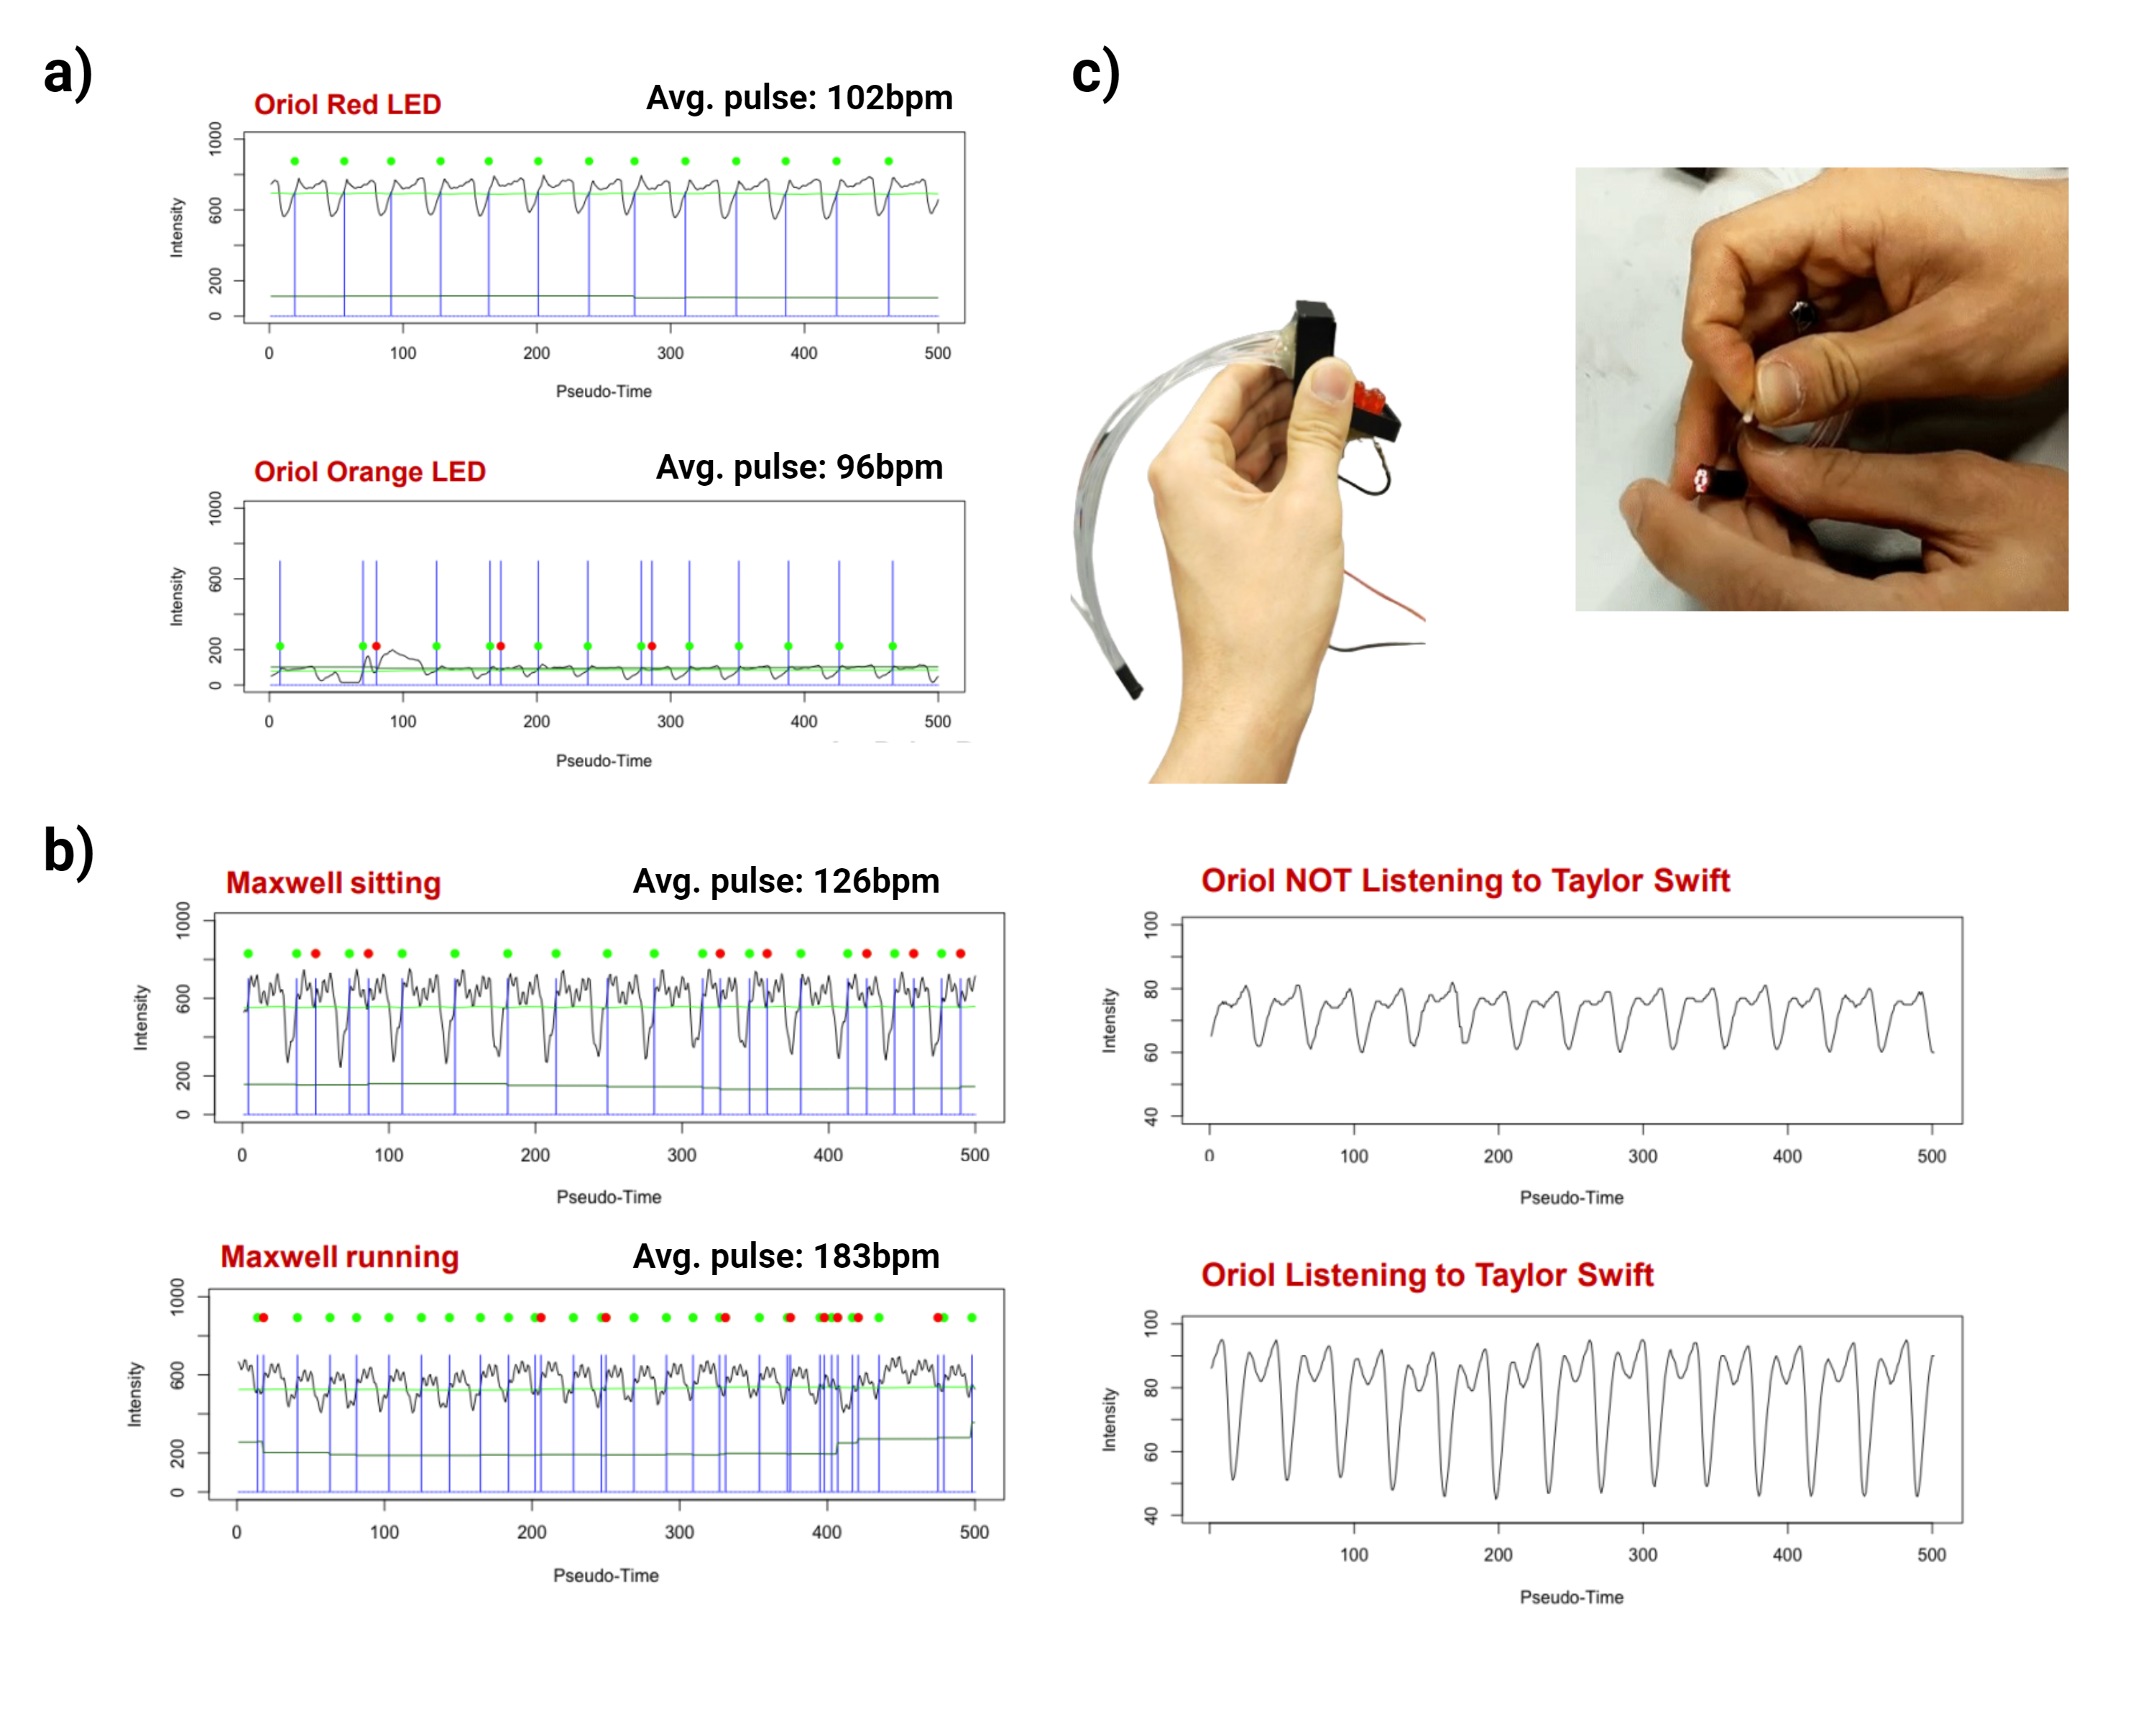
\includegraphics[width=\linewidth]{images/pulse change.png}
         \caption{Characterization of the DIY pulse meter. (a) Red LED allows for better signal detection. (b) Detection of changes in pulse after physical excersice and listening to music with emotional charge. 
         (c) Optic fiber test.}
         \label{fig:pulsechange}
      \end{figure}


      \subsubsection{Results and conclusion}
      The main conclusions we drew from our characterization of the prototype are the following: (a) after trying both red and orange LEDs, 
      we assessed that using red light allows for better amplitude of the signal; (b) our device correctly detect rapid changes in pulse rate as 
      the one experienced when running or listening to music we connect to (Figure \ref{fig:pulsechange}).

      We also noticed that, as the sensor was connected to the main board by a long wire prior to signal amplification, the latter was prone 
      to get electromagnetic noise from the environment. Even if the best solution would be to implement a design where the amplification occurs 
      near the sensor and then the electrical signal moves to the board, we wanted to experiment moving the actual light from the finger to the 
      main board (Where the sensor would be placed) through optic fiber. However this was unsuccessful, as the signal of the optic fiber was not 
      strong enough to be detected by the photodiode (Data not shown). 

      



\bibliographystyle{IEEEtran}
\bibliography{guided_sensor}

% Uncomment the compliance section if you have set it up properly
\section{Compliance}
\wordcount

Words calculated automatically using texcount package on the original LaTeX file.

\newpage
\appendices
\section{Operational amplifier calibration}
\begin{figure}[h]
   \centering
   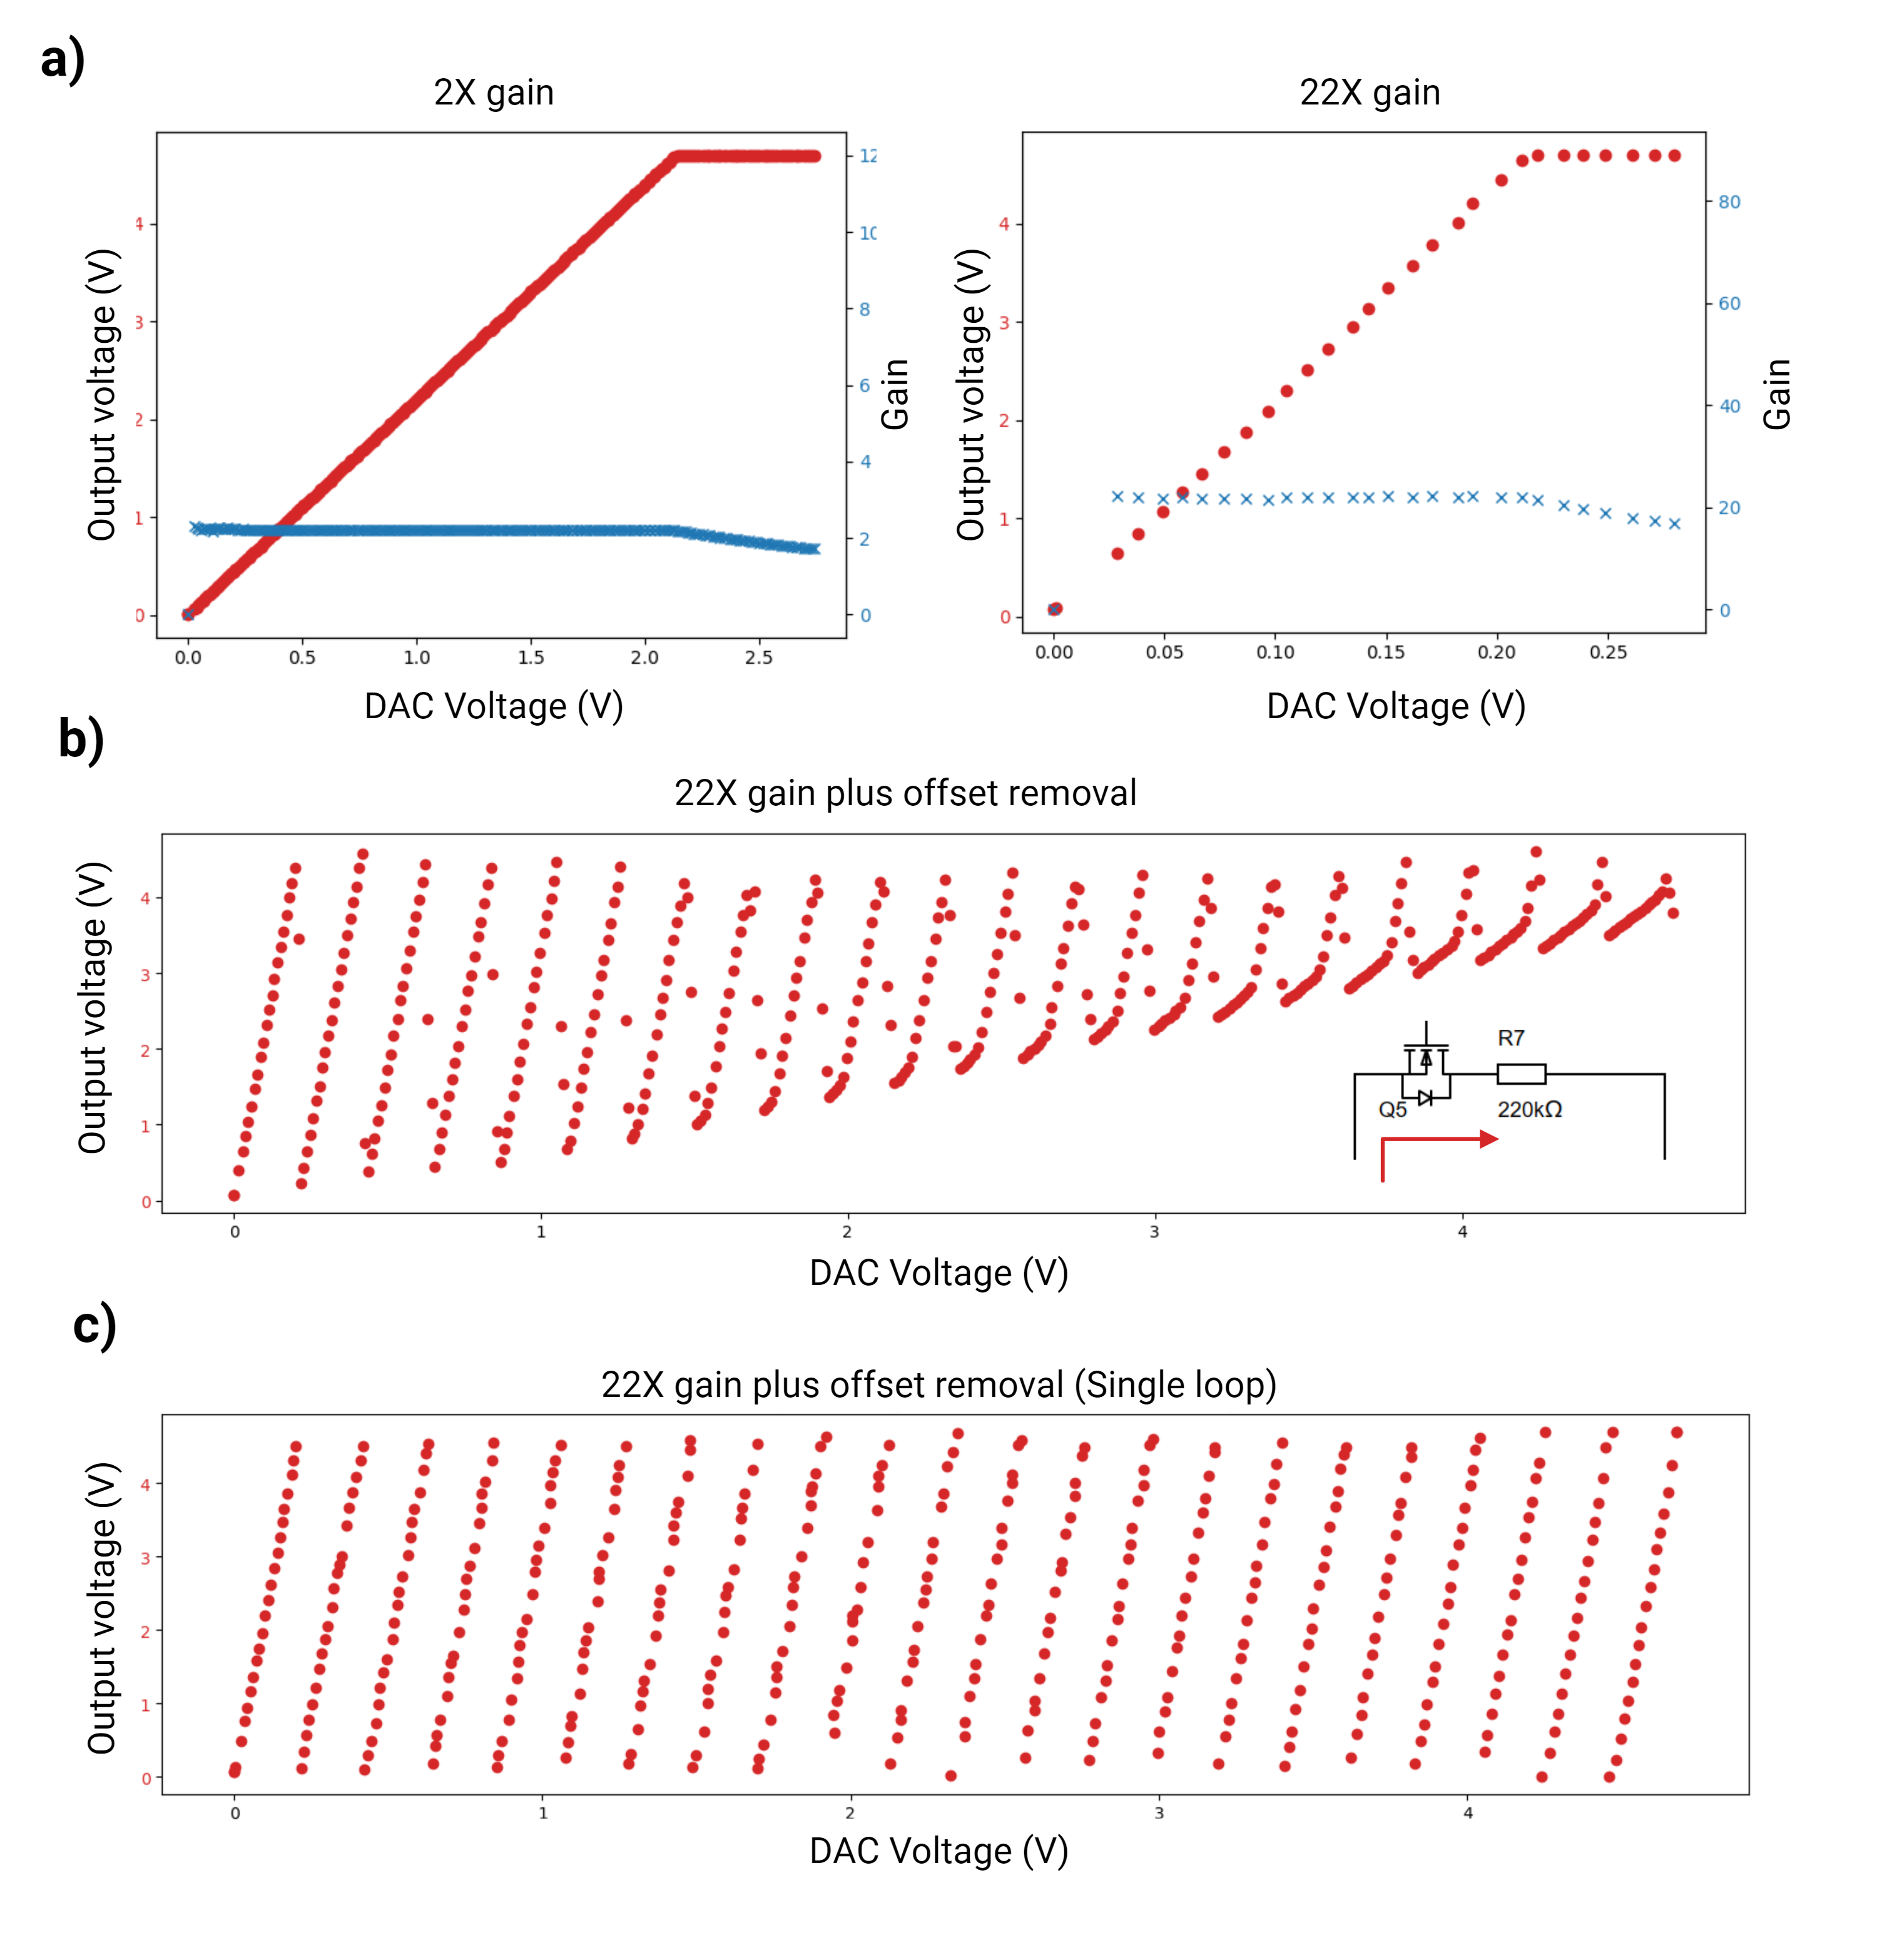
\includegraphics[width=\linewidth]{images/op amp calibration.png}
   \caption{Operational amplifier calibration. Demonstration of the closed-loop resistance exchange circuit without offset removal (a).
   Introduction of offset removal and the appearance of a minimum reachable voltage (b), which is resolved upon removing the MOSFET from the gain 2 closed-loop (c).}
   \label{fig:opamp}
\end{figure}

\end{document}
